\chapter[Particle Identification and Event Reconstruction]{Particle Identification and Event Reconstruction}
\label{chap:ParticleID}

%PF jet reconstruction is an important key for the search of $Z'$ bosons in the di-hadronic tau channel since 
%jets are used as initial seed for the tau-lepton reconstruction. \\

%The energy of a jet is carried by charged hadrons ($~65 \%$), photons 
%from $\pi^{0}$ decays ($~15 \%$) and neutral hadrons ($~20 \%$) \cite{CMS-PAS-PFT-10-001}. \\


\section{Particle Flow}
\label{sec:PF}

The Particle Flow (PF) algorithm \cite{CMS-PAS-PFT-09-001} identifies and reconstructs all the stable-visible particles produced in the hard interaction, by
combining the information collected by the CMS sub-detectors in order to optimize the determination of their direction, energy and type. The PF 
technique performs the global event reconstruction classifying all the visible particles into five mutually exclusive groups: photons, 
neutral hadrons, charged hadrons, electrons and muons. This list of individual particles (called ``PF Candidates'') are used 
as an input in further algorithms to reconstruct higher level objects such as jets, missing transverse energy and tau-leptons. \\

%The capabilities of the CMS detector are ideal for using the PF technique as a global event reconstruction. The high 
%granularity of the inner tracker and the ECAL, the hermiticity of the HCAL, the high performance of the muon system 
%along with the strong magnetic field provided by the superconducting solenoid allow PF technique to reach a 
%high performance reconstruction for the individual particles produced in the hard interaction, even for charged particles
%with very low $\textrm{p}_{\textrm{T}}$ of an order of 100 MeV; this leads to an improvement in the energy jet corrections. Besides, the high performance of the individual particle reconstruction 
%allows to discriminate between nearby tracks such as the decay products of the tau-lepton. The main advantage 
%to use the PF technique as a global event reconstruction is the high performance reconstruction 
%for all the physics objects, in particular jets, MET and tau-leptons \cite{CMS-PAS-PFT-10-001}.\\


The capabilities of the CMS detector are ideal for using the PF technique as a global event reconstruction. The high 
granularity of the inner tracker and the ECAL, the hermiticity of the HCAL, the high performance of the muon system 
along with the strong magnetic field provided by the superconducting solenoid allow PF technique to reach a 
high performance reconstruction for the individual particles produced in the hard interaction, even for charged particles
with very low $\textrm{p}_{\textrm{T}}$ (of the order of 100 MeV). This leads to an improvement in the global event 
reconstruction since, instead of using special sub-detectors designed to reconstruct an specific 
object (like alternative event reconstruction techniques), PF algorithm uses a more completed information collected 
by all CMS sub-detectors, avoiding any ambiguity to reconstruct the object. Besides, the 
individual particle reconstruction provides a detailed information 
about compositeness of high level objects like jets, allowing PF technique
to determinate the hadron profile of the jet and its origin, which is important for the tau-identification. 
Additionally, the high performance of individual particle reconstruction allows to discriminate between nearby tracks 
such as the decay products of the tau-lepton. The main advantage 
to use the PF technique as a global event reconstruction is the high performance reconstruction 
for all the physics objects, in particular jets, MET and tau-leptons \cite{CMS-PAS-PFT-10-001}.\\

%and the ECAL, the hermicity of the HCand clusters with high efficiency.

The PF technique is performed in three steps: First, the algorithm builds the so-called ``PF elements'' which consist of tracks 
reconstructed in the Inner Tracker, energy clusters reconstructed in the calorimeters and tracks observed in the muon system \ref{sec:MuonSys};
the second stage addresses the topological association of the basic PF elements each other using the ``link-algorithm''; finally,
individual particles are identified and reconstructed from the content of the linked elements. \\

%Photons are reconstructed from its energy deposits in the ECAL (See section \ref{sec:Photon});
%electrons are reconstructed by the combination of tracks and the energy deposits in the ECAL of the electron itself and the 
%Brestrahlung radiation produced by its interaction with the tracker material (See section \ref{sec:Electron}); Muon reconstruction 
%is performed connecting together the tracks reconstructed by the inner tracker and the muon system, it will be described in section \ref{sec:Muon};

\subsection{Track Reconstruction}
\label{subsec:TrackReco}
The track reconstruction in the inner tracker is one of the most important keys of the global event reconstruction. The inner tracker, due to its
high granularity, provides a precise reconstruction of the charged-particle tracks and consequently give rise to an accurate reconstruction 
of the primary vertex, identifying it from the pileup interactions. \\

The track reconstruction is performed in several steps by a process called \textit{iterative tracking}. In the initial iterations, 
the iterative tracking applies a tight criteria in order to search for tracks easy to identify (tracks 
with relative high $\textrm{p}_{\textrm{T}}$ produced near the interaction region). In the next iterations, the hits 
unambiguously assigned to a track are removed. This reduces the combinatorial complexity in the subsequent iterations 
and allows to loosen the selection criteria to identify the tracks associated with low $\textrm{p}_{\textrm{T}}$. In the first three iterations, 
the iterative tracking reaches an efficiency up to 99.5$\%$ for isolated muons and larger than 90$\%$ for 
charged hadrons in jets \cite{CMS-PAS-PFT-09-001}. Last iterations relaxes the constrains on the origin of the vertex 
to find tracks originated outside the beam spot (secondary charged particles from photon conversions in the tracker material) 
and to reconstruct the remaining tracks. Each iteration could be summarized in 4 steps:\\

\begin{itemize}
 \item Tracks are seeded using 2 or 3 hits, giving rise to the initial track candidates and their initial trajectory parameters.
 \item The track finder algorithm is based on the Kalman filter \cite{Fruhwirth:1987fm}, which consist in an extrapolation outwards of the inner 
       tracker layers with the purpose to find additional hits associated to the track and to estimate the track 
       parameters. The filter recalculates the track parameters for each layer, accounting the energy loss and the 
       multiple Coulomb scattering produced by the interaction of the charged particle and the tracker material.
 \item A fit on the track is performed to estimate all the possible information of the trajectory.
 \item Tracks are selected on basis of the quality flags, whether they are compatible with some 
 criteria such as $\chi^{2}$ and if they are originated from the primary vertex.
\end{itemize}

The efficiency estimation of the track reconstruction is performed comparing the reconstructed tracks with MC samples which 
contains just single muons or pions. Muons are ideal for this purpose since muons, unlike electrons, have a negligible energy loss
through bremsstrahlung radiation due to the interaction with the tracker material. Unlike muons, charged pions (a possible tau decay product) do not 
only undergo Coulomb scattering but it (as all hadrons) also loses energy though strong interactions with the tracker material. These nuclear 
interactions are not taken into account in the track Finder algorithm, reducing the track reconstruction efficiency in the tracker acceptance. The tracking efficiency 
is higher than 99$\%$ for isolated muons with a $\textrm{p}_{\textrm{T}}>1$ $\textrm{GeV}$ while for charged pions is close 
to 95$\%$ for $\textrm{p}_{\textrm{T}}>1$ $\textrm{GeV}$ \cite{Chatrchyan:2014fea} (See Figure \ref{fig:Track_Efficiencies}). The PU interactions
degrades significantly the tracking efficiency for tracks with $\textrm{p}_{\textrm{T}}<1$ $\textrm{GeV}$ \cite{Chatrchyan:2014fea}. Efficiencies 
were obtained from 2011 data for pp collision at a centre-of-mass energy of $\sqrt{s} =$  7 TeV. For simulated events an average of 8 for pileup interactions was used, which corresponds
roughly to the amount delivered by the LHC on 2011.


%The tracking
%efficiency depends, besides on the $\textrm{p}_{\textrm{T}}$, on $\eta$ due the geometrical acceptance of the tracker and 
%the PU which degrades the efficiency for tracks with $\textrm{p}_{\textrm{T}}<1$ $\textrm{GeV}$




\begin{figure}[ht]
  \begin{center}
    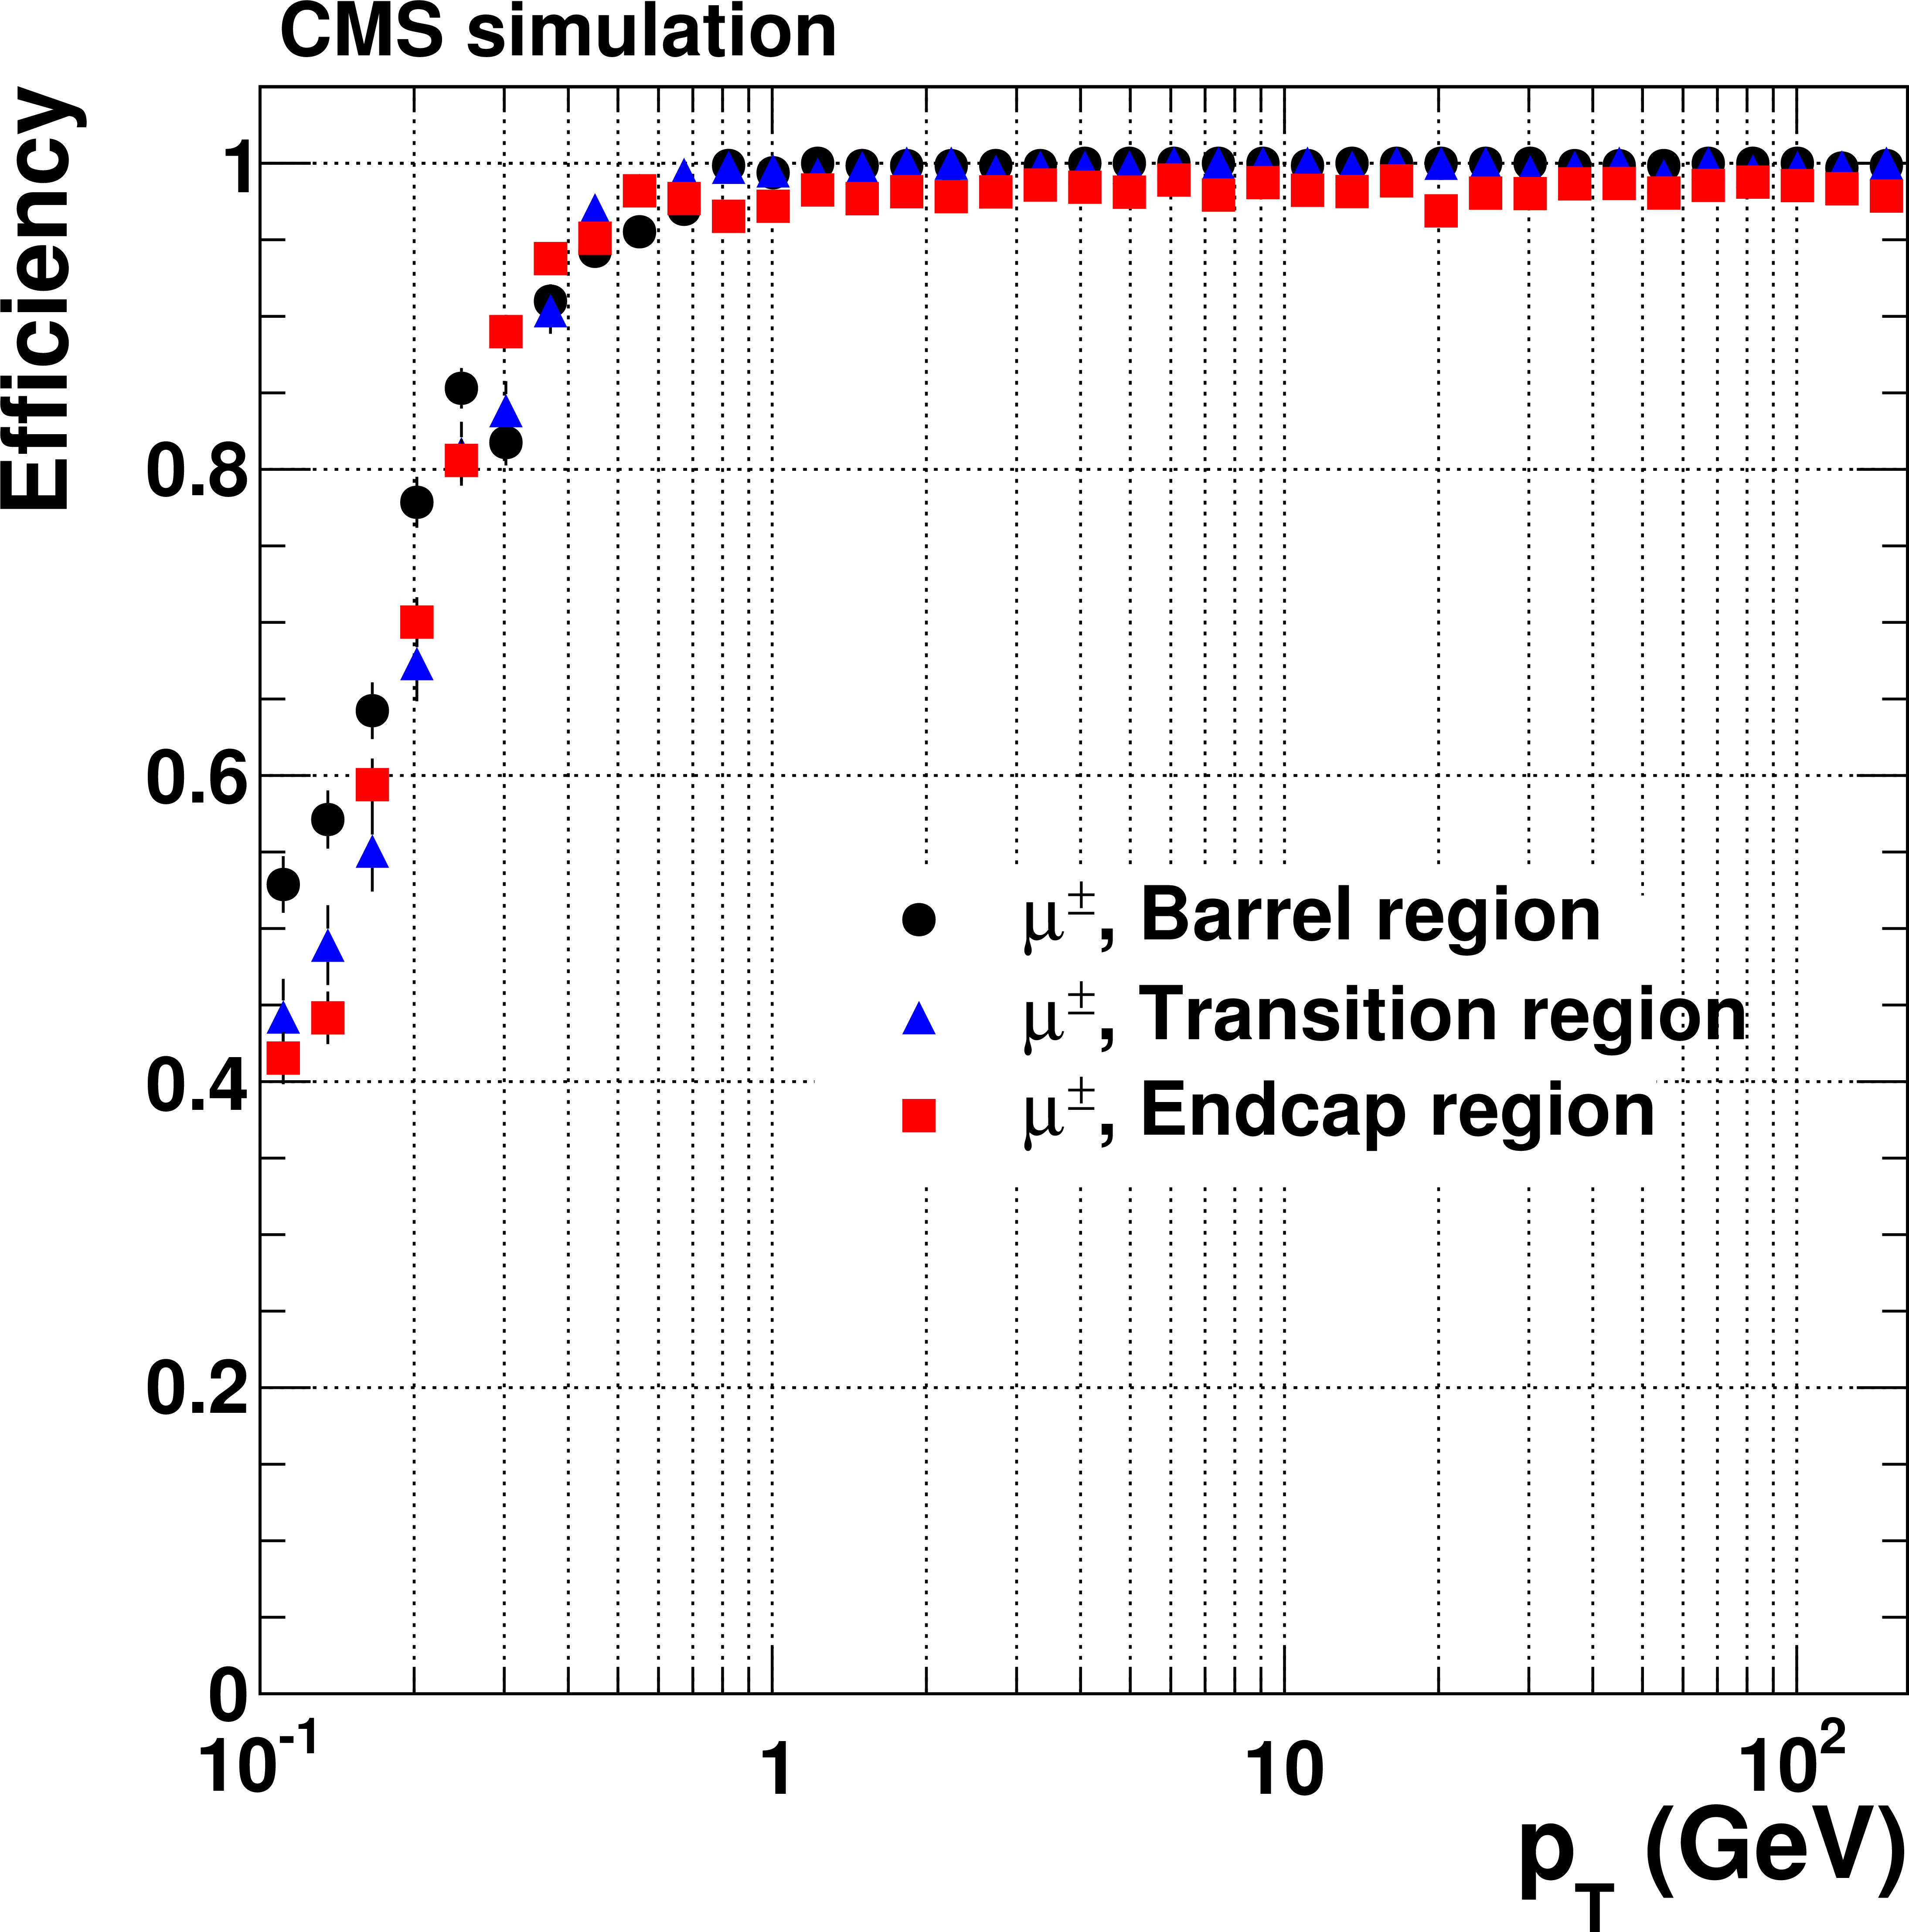
\includegraphics[width=0.35\textwidth]{figuras/Chapter3/TrackEff_Muon_pt.png}
    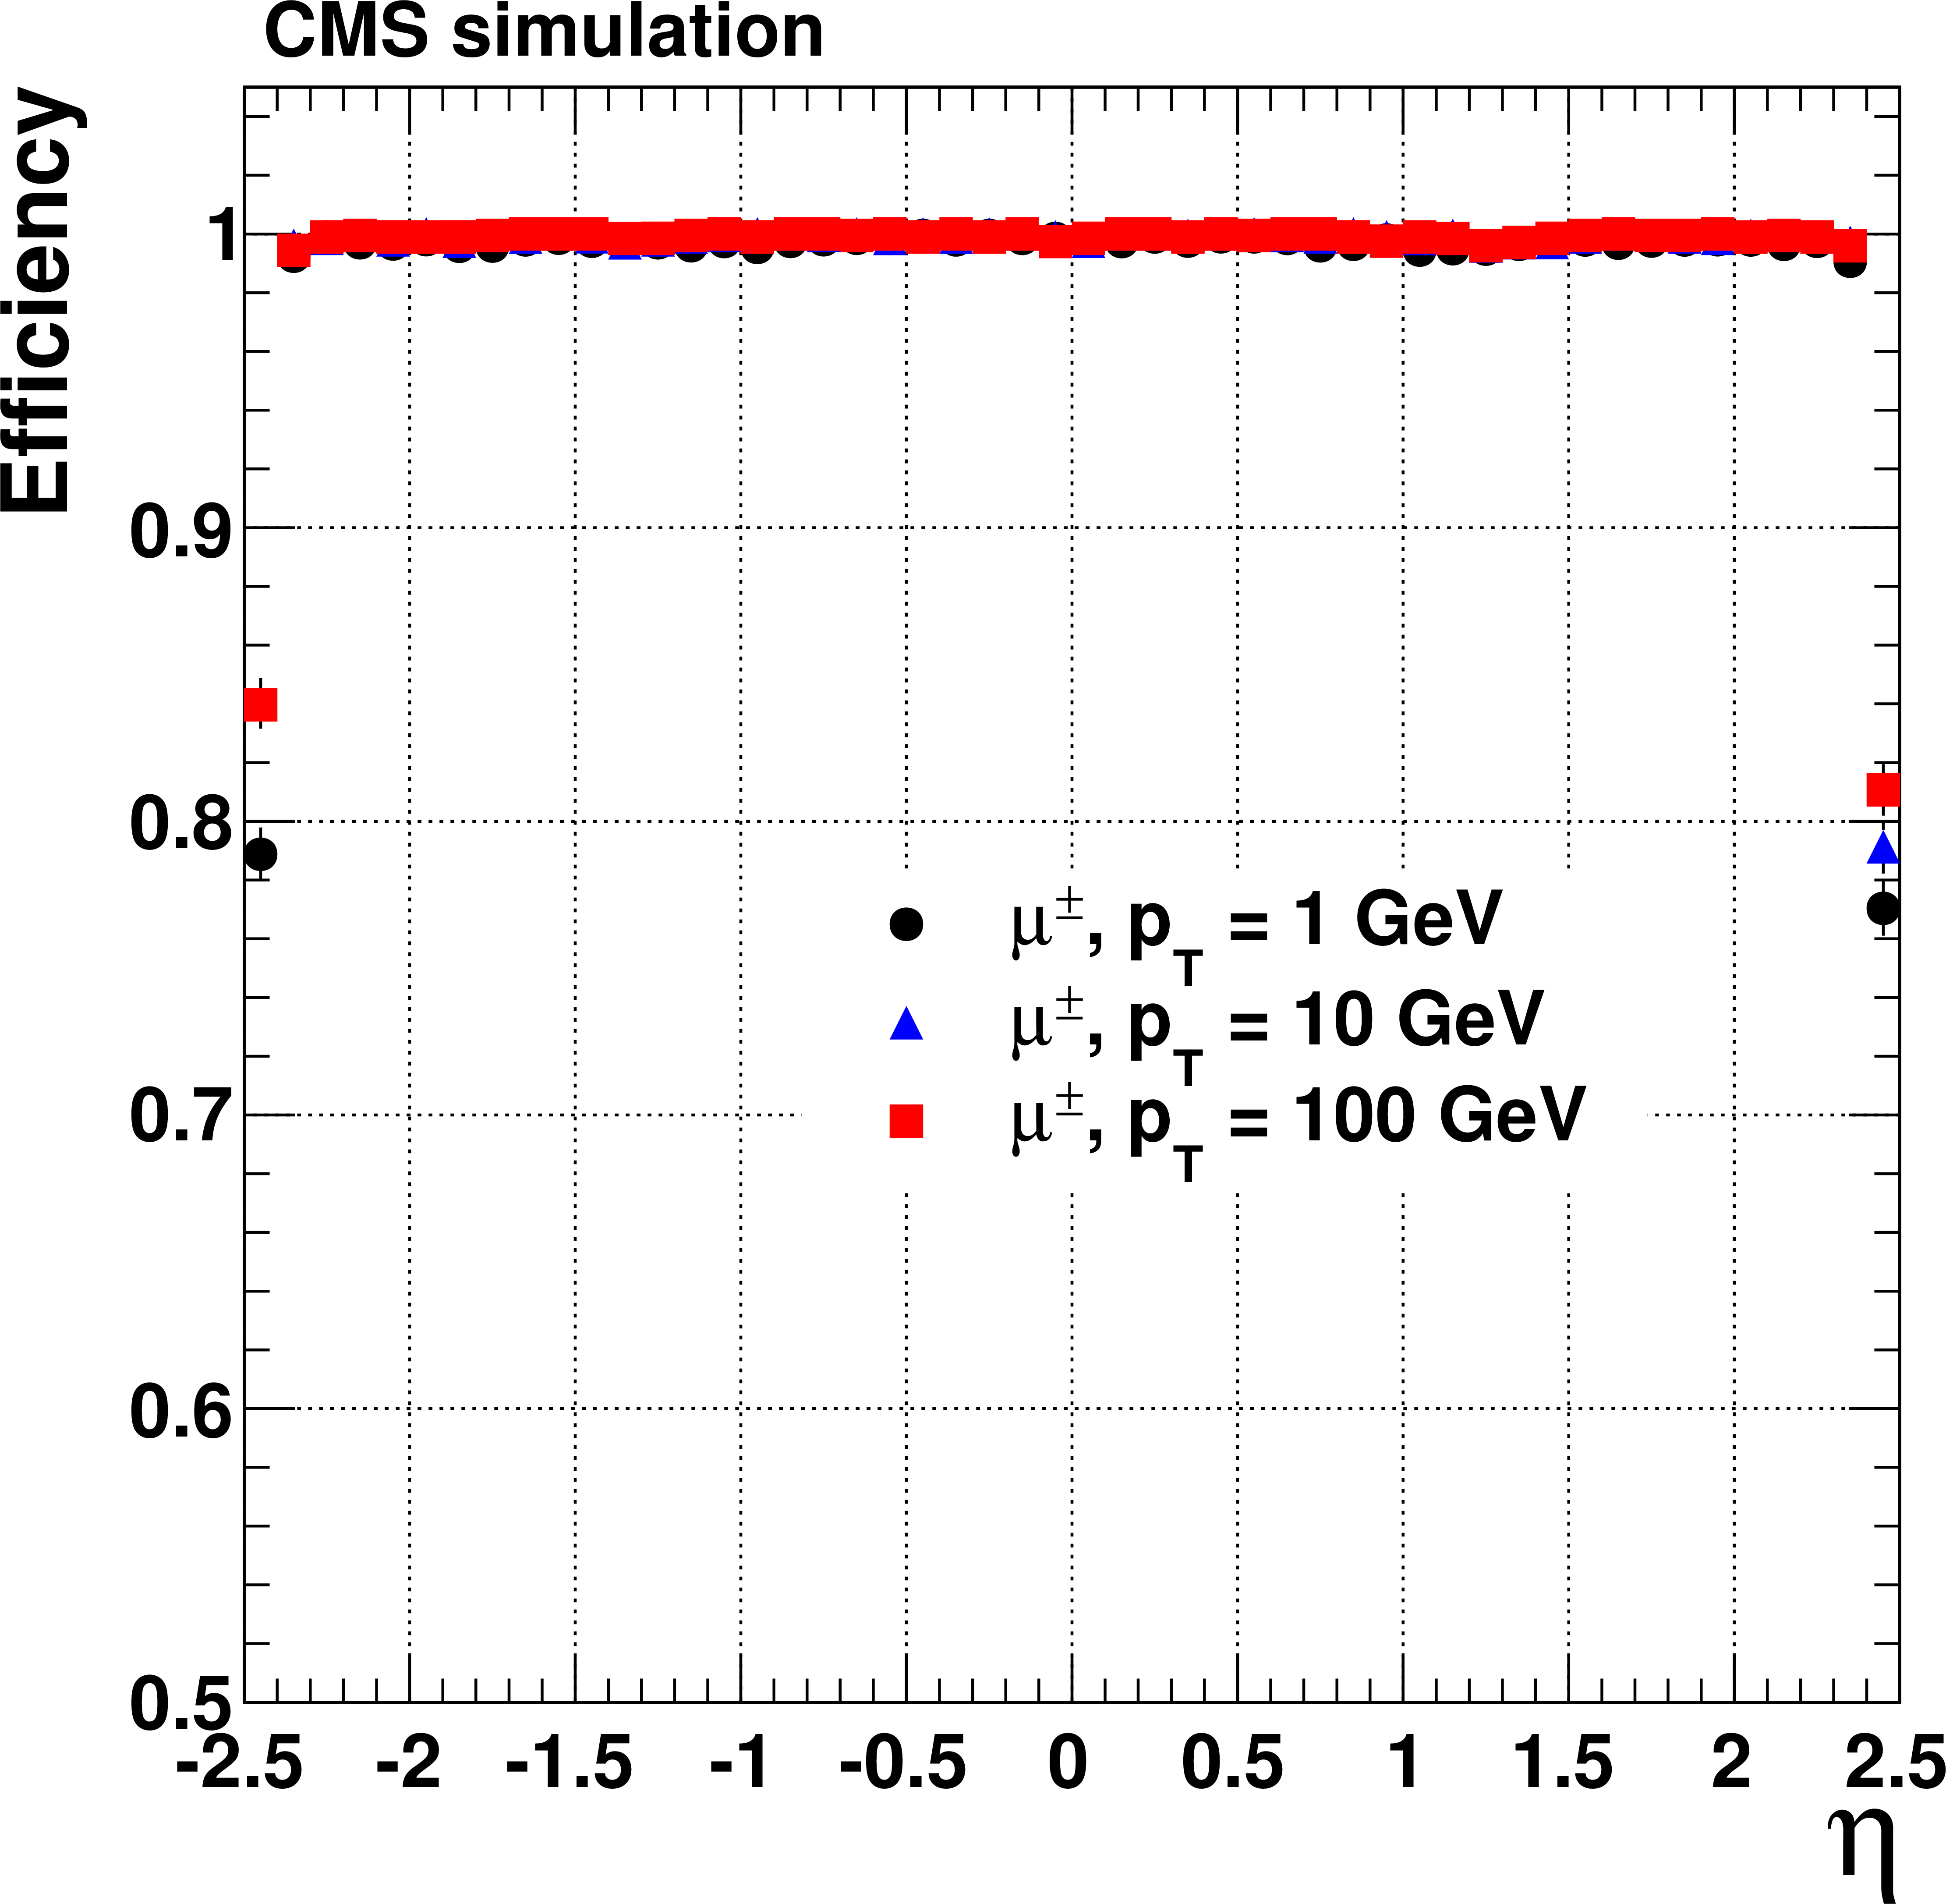
\includegraphics[width=0.35\textwidth]{figuras/Chapter3/TrackEff_Muon_eta.png}
    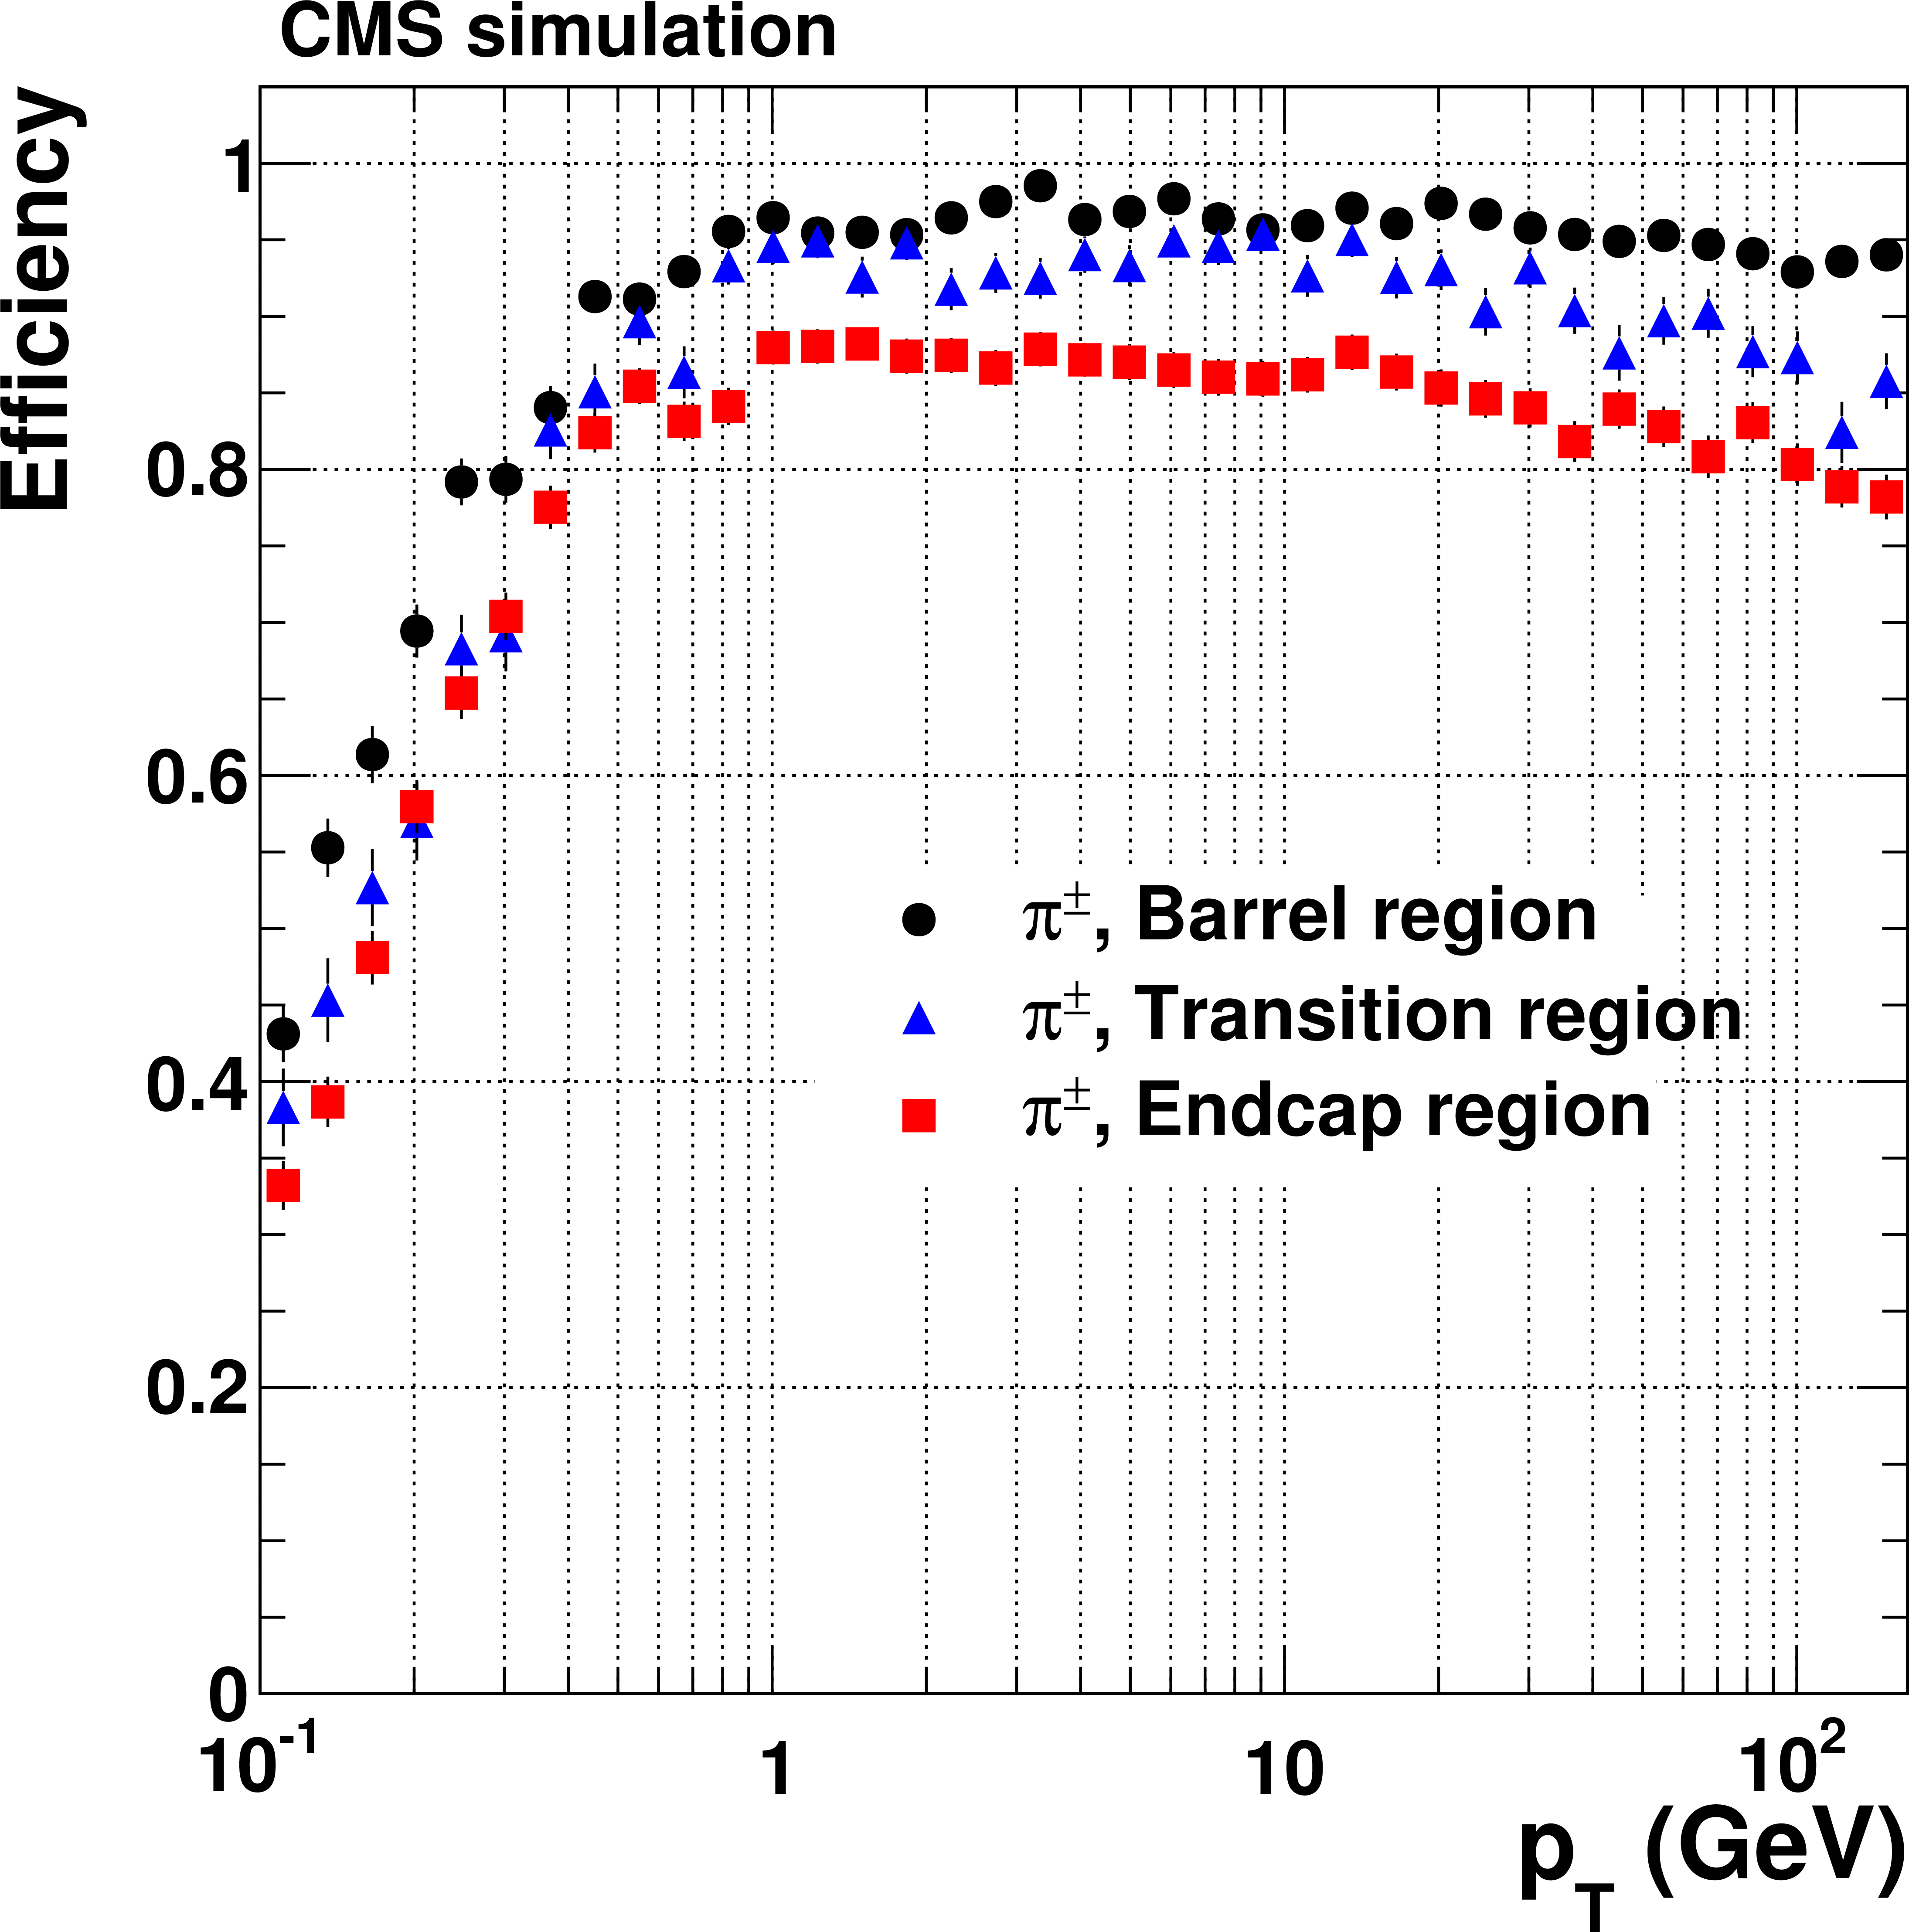
\includegraphics[width=0.35\textwidth]{figuras/Chapter3/TrackEff_Pion_pt.png}
    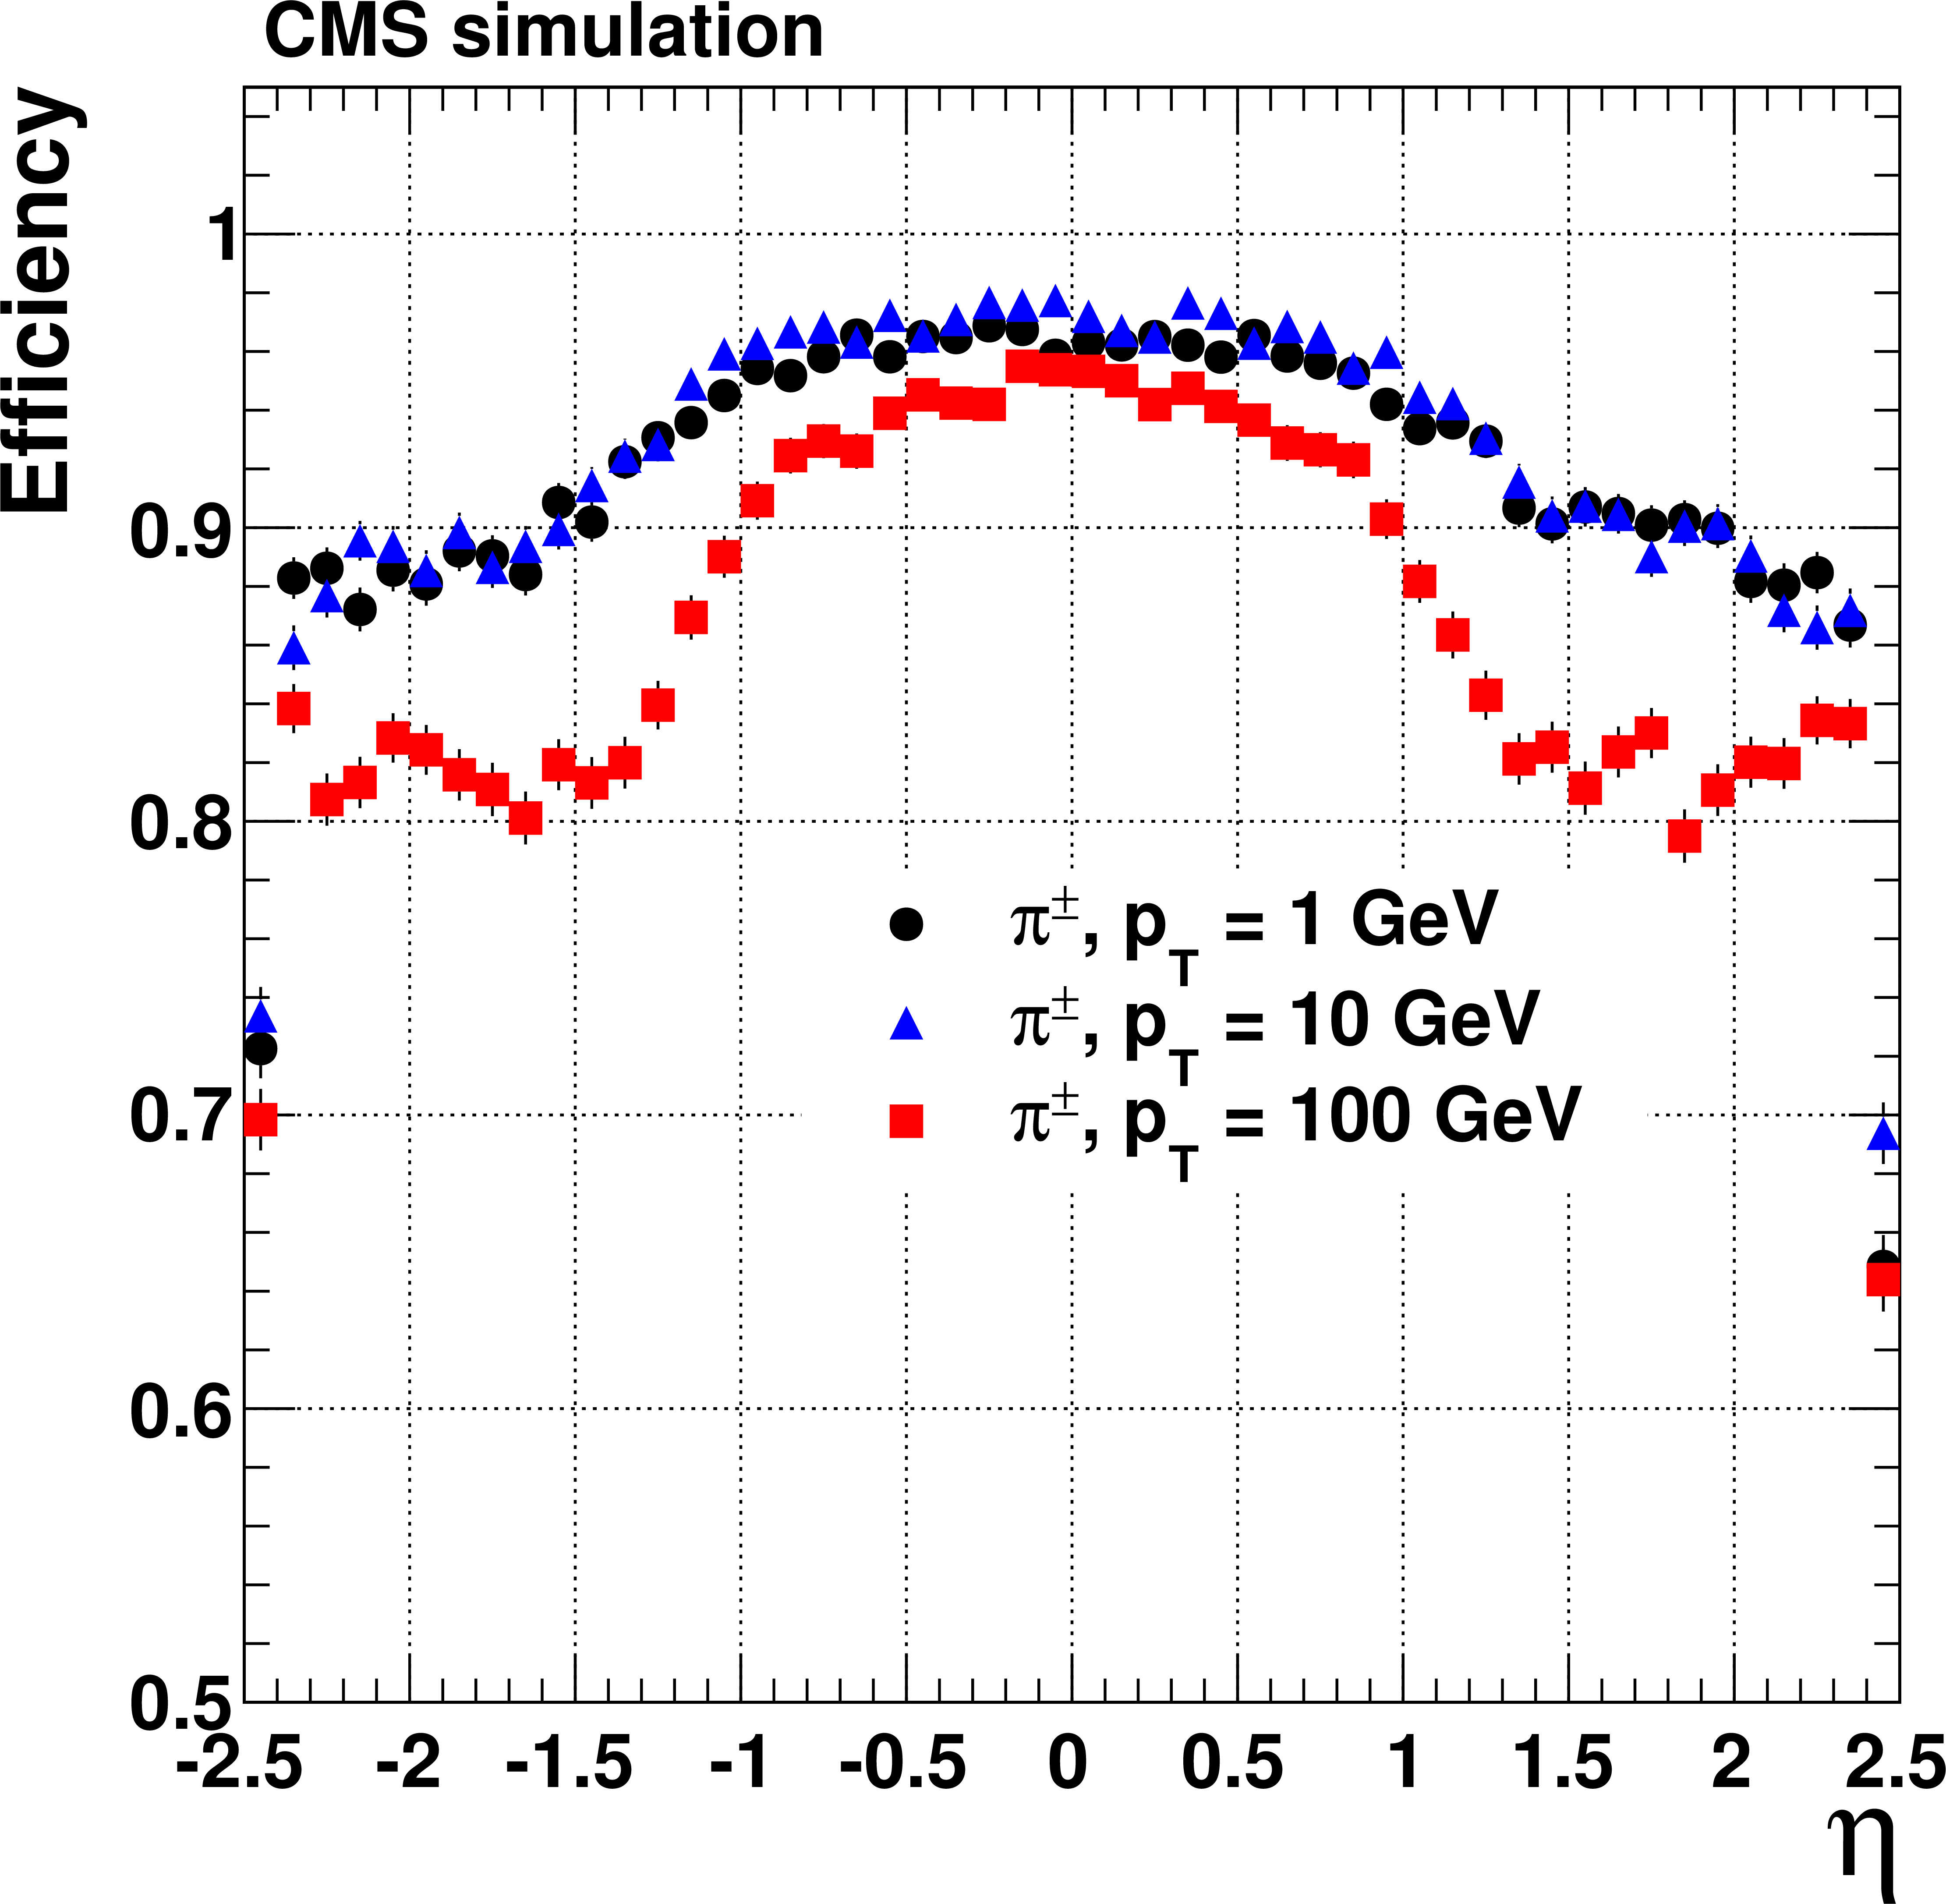
\includegraphics[width=0.35\textwidth]{figuras/Chapter3/TrackEff_Pion_eta.png}
    \caption{Efficiency of reconstructed track as function of $p_{\textrm{T}}$ and $\eta$ for 
    muons (top) and charged pions (bottom). Efficiencies were obtained using pp collisions with a centre-of-mass 
    energy of $\sqrt{s} =$  7 TeV, which corresponds to 2011 data. For simulated data an average of 8 pileup 
    events was used, which is roughly the amount delivered by the LHC on 2011. Figure taken from \cite{Chatrchyan:2014fea}}
    \label{fig:Track_Efficiencies}
  \end{center}
\end{figure}

\subsection{Vertex Reconstruction}

%Primary vertex reconstruction is performed with the purpose to measure the position, and the uncertainty, 
%of all vertices produced in the pp collisions, such as the vertex produced by a hard interaction, secondary 
%vertices coming from b-jets as well as pileup collisions. Vertex reconstruction first proceed with a 
%track selection, then reconstructed tracks are clustered to identify vertices, and finally the vertex position
%is determined by a fit. \\

Primary vertex reconstruction is performed with the purpose to measure the position, and the uncertainty, 
of all vertices produced in the pp collisions. Vertex reconstruction proceed first with a 
track selection, then reconstructed tracks are clustered to identify vertices, and finally the vertex position
is determined by a fit. The main criteria for track selection are the impact parameter relative to the beam spot, the
number of reconstructed hits in the tracker and the $\chi^{2}$ associated to its trajectory. Then, the 
selected tracks are grouped into clusters according to their z-coordinates with the aim of identifying
all possible vertices even for inelastic collisions. Track clustering is performed with the 
deterministic annealing (DA) algorithm \cite{VertexRecoBIB}. The DA algorithm resolves iteratively
the z-coordinates of all the possible vertices and the cluster of tracks associated to them, in a similar way 
to solve a physical system with many degrees of freedom, approaching iteratively to the state 
of minimum energy \cite{Chatrchyan:2014fea}. Finally, the adaptive vertex fitter technique \cite{Fruhwirth:1027031}
is used in order to perform the best estimation of the vertex parameters, in particular the position,
from fitting the cluster of tracks associated to the vertex. The primary vertex is selected from the vertex with the higher
sum of $\textrm{p}_{\textrm{T}}^{2}$ of the cluster of tracks.\\

The resolution of the primary vertex depends on the number of tracks associated to it. Figure \ref{fig:RecoVertex} 
shows the resolution of x and z position for primary vertex reconstruction, using minimum vias samples 
\footnote{Minimum vias samples pass a suit of triggers and minimum requirements on hit 
or track multiplicity} and jet-enriched data samples \cite{Chatrchyan:2014fea}. The resolution for x and z position 
is, respectively, less than 20 $\mu$m and 25 $\mu$m for the minimum vias samples while it is 
improved to less than 10 $\mu$m and 12 $\mu$m for jet-enriched samples. Figure \ref{fig:RecoVertex} c) shows
the efficiency of primary-vertex reconstruction which depends on the number of tracks. 

\begin{figure}[ht]
  \begin{center}
    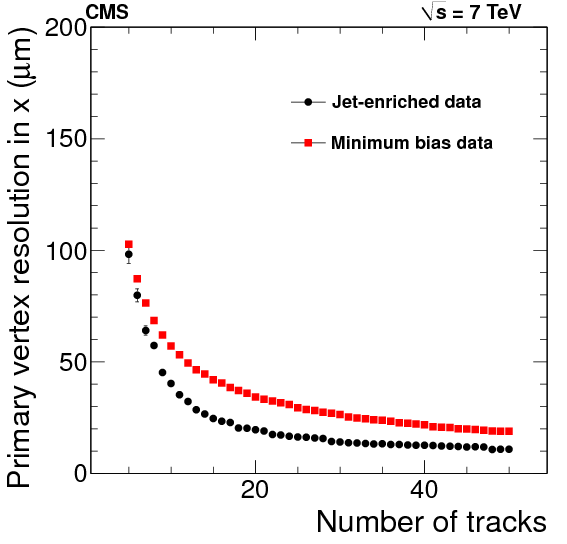
\includegraphics[width=0.3\textwidth]{figuras/Chapter3/RecoVertex_x_resolution.png}
    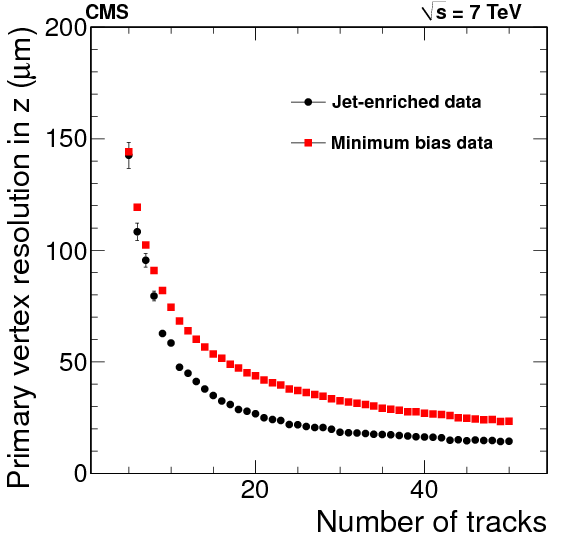
\includegraphics[width=0.3\textwidth]{figuras/Chapter3/RecoVertex_y_resolution.png}
    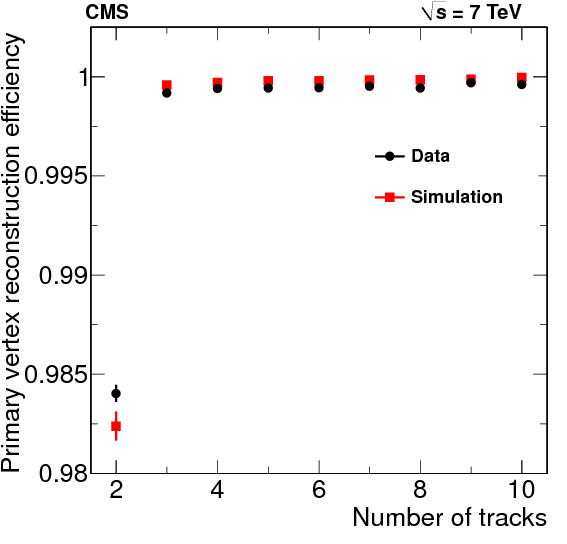
\includegraphics[width=0.3\textwidth]{figuras/Chapter3/Effciiency_vertex_resolution.png}
    \caption{Resolution of x and z position  for primary vertex reconstruction, using a) minimum vias samples and b) jet-enriched samples. 
    Resolution is improved using jet-enriched samples since in these sample the mean of $\textrm{p}_{\textrm{T}}$ is larger than minimum vias samples.  
    For efficiency of primary vertex reconstruction shown in c), minimum vias MC samples were used. Results were estimated 
    with pp collisions with a centre-of-mass energy of $\sqrt{s} =$  7 TeV. Figures were taken from \cite{Chatrchyan:2014fea}.}
    \label{fig:RecoVertex}
  \end{center}
\end{figure}

%El algoritmo lo que hace es buscar la minima temperatura ``T'' local para el cual chi2 sea minima, 
% comienza con T-> inf, todos los tracks estan asociados a un solo vertice, la T comienza a disminuir,
% comienza a crecer el numero de vertices, se hace eso hasta que el sistema alcanza la Tcritica (el punto de inflexion de la energia libre F)
% (chi2 hace las veces de la eneria)
% una vez se encuentra el minimo local, cada vertice se convierte en dos, endonde el peso asociados a esos vertices es igual al vertice ``papa''
% eso se hace iterativamente hasta alcanzar una T igual a 4 en donde ya hay una posibilidad de convertir un real vertice en dos.


\subsection{Clustering}
\label{subsec:Clustering}
Other important part of the PF technique, in addition to the tracks, is the reconstruction of the 
calorimetric clusters. The calorimeter clusters are used to identify the energy deposits which come from 
%neutral-visible particles, such as photons and neutral hadrons, and discriminate them from the energy deposits 
photons and neutral hadrons, and to discriminate them from the energy deposits due charged hadrons; 
besides it reconstructs the electrons along with their associated Bremsstrahlung radiation
and helps to determinate the track parameters of the charged hadrons which were not measured 
accurately from the track reconstruction (for example, charged hadrons that are outside of the tracker acceptance, or 
charged hadrons with high $p_{\textrm{T}}$). The clustering is performed for 
each part of the CMS calorimeter system: ECAL, HCAL, HF and PS.\\

The clustering algorithm proceeds from the ``cluster seeds'' identified at local level. Cluster seeds are selected 
from individual calorimeter cells which have a maximal energy deposits above a given energy. Once the cluster seed is selected,
the algorithm searches for energy deposits in the  boundary cells with a common side. The algorithm aggregates to the cluster 
at least one additional cell with a maximum energy higher than two standard deviations from the electronic noise: 80 $\textrm{MeV}$ in 
barrel and up to 300 $\textrm{MeV}$ in the end-caps for the ECAL, while 800 $\textrm{MeV}$ for the HCAL \cite{CMS-PAS-PFT-09-001}. This
cells combined are known as ``topological clusters''. The topological clusters are taken as ``particle flow clusters'' seeds
in order to solve any overlapping among clusters.

\subsection{Link algorithm}
\label{subsec:Linkalgorithm}
As mentioned earlier, a particle is expected to produce signatures in different sub-detectors, giving rise to one or more 
so-called PF elements: tracks, clusters and tracks in the muon system; for example, 
a charged hadron as the pion, would produce a track in the inner tracker along with 
energy deposits in both calorimeters. PF uses the \textit{link algorithm} to perform a topological combination 
of the PF elements reconstructed in the different sub-detectors with the aim of reconstructing fully each particle in the event. \\
%of the PF elements recontructed in the different subdetectors with the aim of identifying the type of each particle in the event. 

The link between a charged particle track and a calorimeter cluster is performed as follows:

\begin{itemize}
 \item The track is extrapolated from the last hit reconstructed in the tracker to: the two layers in the PS, the expected depth
 for an electron shower in the ECAL and one interaction length for an typical hadron shower in the HCAL. 
 \item The track is linked to a cluster if the extrapolated position in the calorimeter is within the cluster boundaries. 
 \item The distance in the $\eta-\phi$ plane between the extrapolated track position and the cluster position defines the quality of the link. 
\end{itemize}

Similarly, two calorimeter clusters (i.e. links between PS and ECAL clusters or links between ECAL and HCAL clusters) are linked when the 
extrapolated position in the more granular calorimeter (PS or ECAL) is within 
the boundaries of the less granular calorimeter (ECAL or HCAL). For example, the link between the ECAL and HCAL clusters
produced by a pion is established when the extrapolated position from the ECAL is within the HCAL cluster boundary. Finally, the 
link between a charged particle track reconstructed in the tracker and a track in the muon system (known as global muon) 
is established by a global fit between the two tracks and its $\chi^{2}$ defines the quality of the link.  

\section{Jets Reconstruction}
\label{sec:Jet}

Quarks and gluons produced by the pp collisions at parton level have a defined color charge, and 
due to the confinement of the strong interaction they can not exist as free particles, instead they 
will follow a process of fragmentation and combination with quarks and gluons from the vacuum to form 
colourless bound states called hadrons; this process is known as hadronization. The hadronization will 
give rise to showers of stable particles which propagate in a localized area. These stable particles 
are detected and from their tracks or energy deposits, they are further clustered into so-called jets (See Figure \ref{fig:JetScketch}). The aim 
of a jet reconstruction algorithm is to determinate the kinematics of the origin of the jet, this is reached with the PF 
technique since it reconstructs all the particles individually from the information collected by CMS sub-detectors
and then cluster them into the jet, making possible the determination of the compositeness and further the origin of the jet.\\


\begin{figure}[ht]
  \begin{center}
    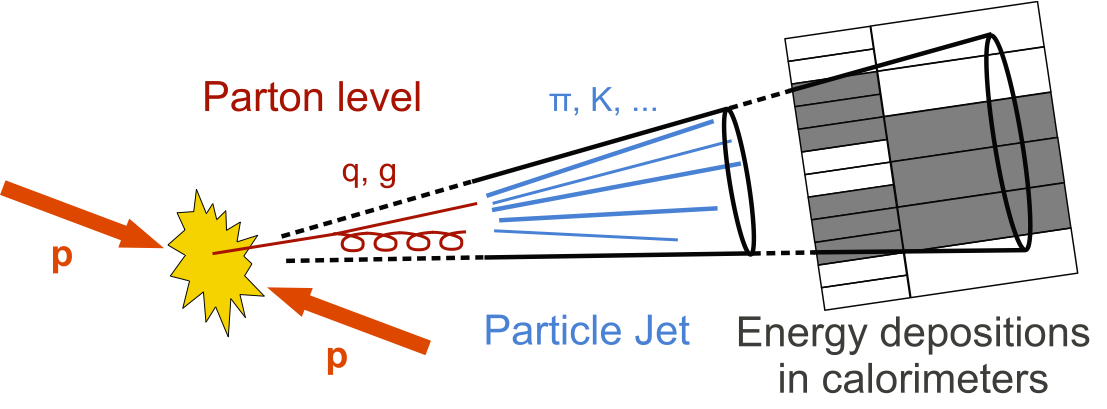
\includegraphics[width=0.6\textwidth]{figuras/Chapter3/JetSketch.png}
    \caption{Schematic diagram of the evolution and detection of a jet.}
    \label{fig:JetScketch}
  \end{center}
\end{figure}


%further reconstructed and finally clustered into so-called jets. The aim of a jet reconstruction 

For the jet reconstruction, the algorithm must consider the jet size. The jet particles are expected to be located 
roughly into an area of $\pi R^{2}$ where $R$ corresponds to the radius parameter of the algorithm. The jet 
area determinates the sensitivity of the jet to soft radiation since if the $R$ parameter is large enough,
all possible particles coming from the hadronization are included in the jet reconstruction,
but also contributions from underlying events (UE) or pileup collision (PU) might be included; this leads to 
an overestimation in the jet energy. \\

The other important qualities to be considered by the algorithm are the infrared and collinear safety (ICR). Infrared 
and collinear processes refers, respectively, to soft QCD radiation and to parton splitting into collinear 
components. If the algorithm is unsafe under these processes, soft radiations will be added to the jet reconstruction
altering the jet components while parton splitting will lead to reconstruct a different number of jets.\\

There are two different types of algorithms that have been used to reconstruct the jet: cone algorithms (SISCone)
and sequential clustering algorithms (kT, Cambridge-Aachen, anti-kT). The main difference between them 
is the way how the particles that belong to a jet are clustered. Cone algorithms consider that the particles 
in a jet will spread out in a rigid conical region which results in an a fixed definition on the jet area, while 
sequential algorithms assume fluctuations on the jet area which boundary is defined with a fixed maximum radius. 
A brief description of the most common used ICR safe algorithms is presented:

\begin{itemize}
 \item The \textbf{SISCone} algorithm \cite{Salam:2007xv} checks all the particles in the event in order to identify stable combinations
 that are coherent with a jet; it searches for a stable cone that contains all the particles associated to a jet and 
 which axis corresponds to the sum of their momentum. The algorithm searches iteratively particles that are 
 contained within a circle in the $\eta-\phi$ plane until a particle matches with the 
 circumference of the cone. The matches are defined as stable cones. Then the particle is removed from 
 the list and the procedure is performed again until no more stable cones are found. Finally stable cones are split or merged
 to reconstruct the jets.
 %i.e. the axis of the cone which contains the particles must be .0

 \item \textbf{kT} algorithm \cite{Ellis:1993tq} estimates the following distance variable for all pair of particles ($i,j$):
 \begin{equation}
  \label{eq:kt}
   d_{ij}=min(p_{Ti}^{2},p_{Tj}^{2})\Delta R_{ij}^{2}/R^{2} 
  \end{equation}
where $\Delta R_{ij}^{2}=\Delta(\eta_{i},\eta_{j})^{2}+\Delta(\phi_{i},\phi_{j})^{2}$ is the distance between particles $i$ and $j$
in the $\eta-\phi$ plane and $R$ is the radius parameter that defines the size of the jet. Other distance variable estimated
in the algorithm is the distance between the beam axis and the particle $i$, defined as $d_{iB}=p_{Ti}^{2}$. Then, the algorithm
proceeds by finding the minimum distance between $d_{ij}$ and $d_{iB}$. If $d_{ij}$ is a minimum, the pair of particles $i,j$ 
are recombined adding their four-momenta and are removed of the list of particles. If $d_{iB}$ is a minimum, the algorithm
identify the particle $i$ as a jet. The distances are recalculated iteratively until all particles are part of a jet.
 
 \item The \textbf{Cambridge-Aachen} algorithm \cite{Atkin:2015msa} proceed similar to the kT algorithm, but defining the variable distance:
 \begin{equation}
  \label{eq:antikt}
  d_{ij}=\Delta R_{ij}^{2}/R;\; d_{iB}=1
 \end{equation}
 Since $d_{ij}$ is independent of the momentum, the jet size will not be clearly defined and UE and PU processes will be included in the jet reconstruction.
 In spite of that this algorithm is used since it allows to determine the jet compositeness.
 
 \item The \textbf{anti-kT} algorithm \cite{AntiKTAlgorithm} defines the distance variables as:
 \begin{equation}
  \label{eq:antikt}
  d_{ij}=min\left(\frac{1}{p_{Ti}^{2}},\frac{1}{p_{Tj}^{2}}\right)\Delta R_{ij}^{2}/R^{2};\; d_{iB}=\frac{1}{p_{Ti}^{2}}
 \end{equation} 
 The anti-kT algorithm follows the same procedure of the kT algorithm: it calculates iteratively the variables $d_{ij}$ and $d_{iB}$
 and searches the minimum of the set ${d_{ij},d_{iB}}$, identifying a jet as the smallest $d_{iB}$ distance. Since 
 the anti-kT $d_{ij}$  variable is dominated by high $p_{\textrm{T}}$ particles, the algorithm will first merge them, resulting in an
 accurate jet area estimation. 
\end{itemize}

CMS and ATLAS uses mainly the anti-kT algorithm although Cambridge-Aachen is also used for many CMS analysis. The advantage for using 
anti-kT algorithm is related with the jet area safety. As mentioned above, the anti-kT algorithm prefers to calculate first the distance
for high $p_{\textrm{T}}$ particles and then, recalculate it including low $p_{\textrm{T}}$ particles. This results in a slightly 
fluctuation in the jet area which is important for removing any contribution from UE and PU processes. The jet area profile for the
explained algorithms are shown in the Figure \ref{fig:JetsAlgos}. \\

\begin{figure}[ht]
  \begin{center}
    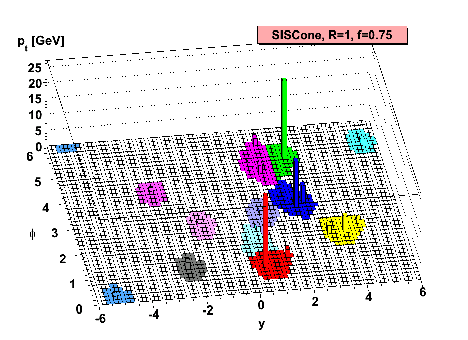
\includegraphics[width=0.43\textwidth]{figuras/Chapter3/herwig-parton-level-ev-siscone-R1-0-f0-75-ghosted4root.png}
    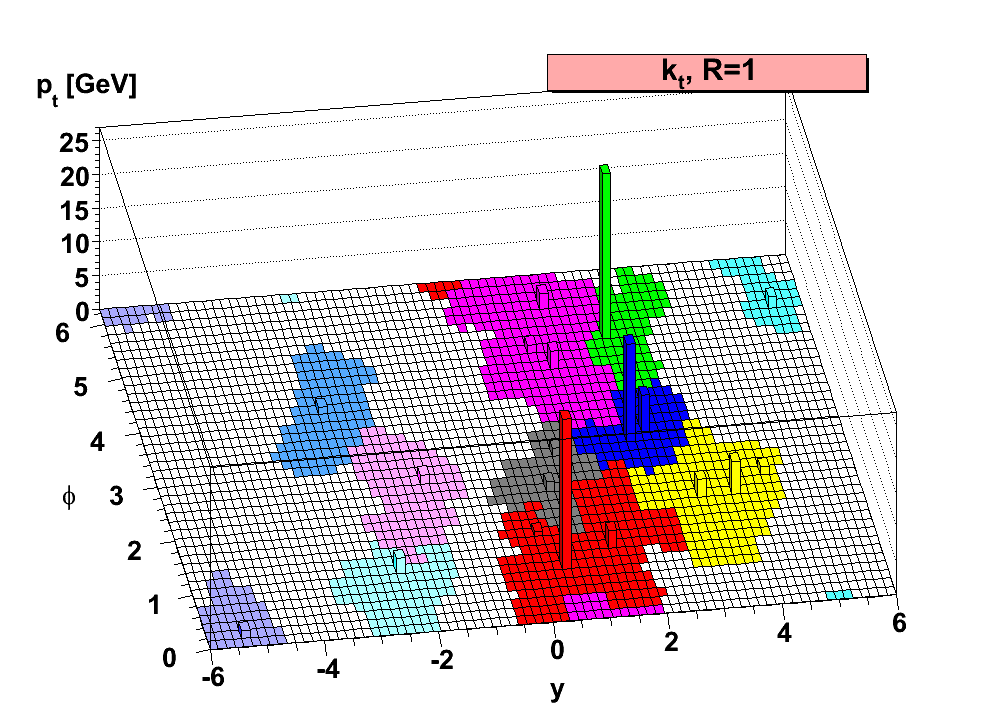
\includegraphics[width=0.43\textwidth]{figuras/Chapter3/herwig-parton-level-ev-kt-R1-0-ghosted4root.png}
    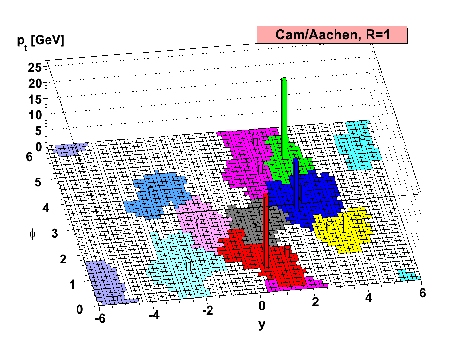
\includegraphics[width=0.43\textwidth]{figuras/Chapter3/herwig-parton-level-ev-cam-R1-0-ghosted4root.png}
    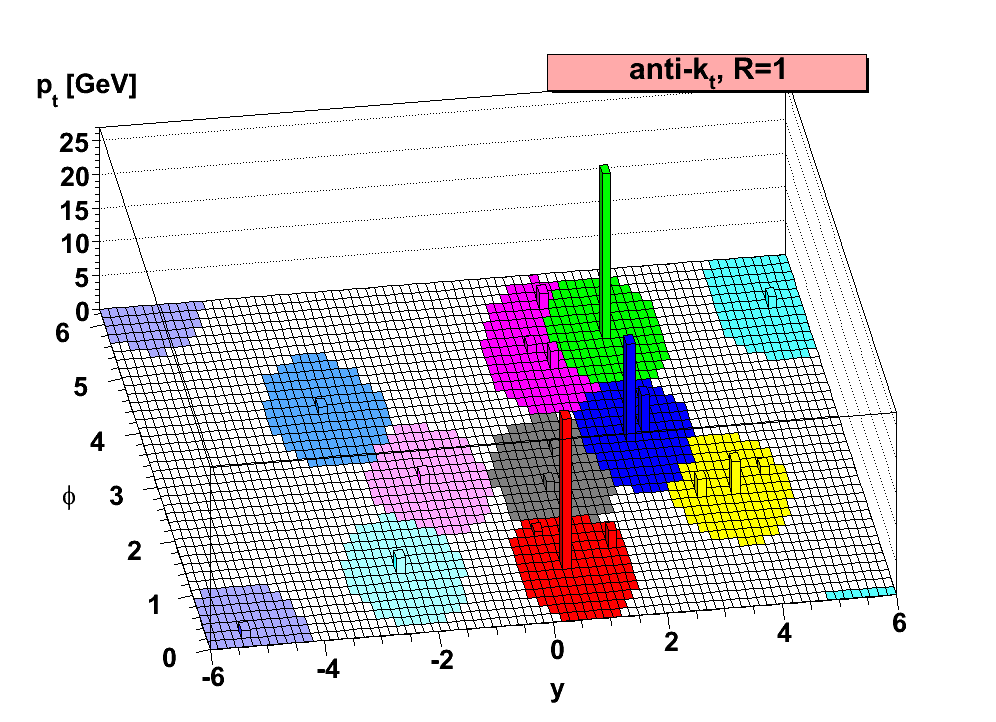
\includegraphics[width=0.43\textwidth]{figuras/Chapter3/herwig-parton-level-ev-antikt-R1-0-ghosted4root.png}
    \caption{Jets reconstruction using the algorithms SISCone (left-up), kT (right-up), Cambridge-Aachen 
    (left-down) and anti-kT (right-down). Jet reconstruction was performed with MC samples using the same $R$
    for all the algorithms. kT and Cambridge-Aachen jet reconstruction show an irregular jet area, while SISCone
    reconstructs jets in smaller areas but identifies two different jets instead of the one grey jet \cite{Atkin:2015msa}.}
    \label{fig:JetsAlgos}
  \end{center}
\end{figure}

%The PF technique \cite{CMS-PAS-PFT-09-001} takes the information collected by the CMS sub-detectors in order to identify and reconstruct
%all the visible final-state particles (electrons, muons, photons, charged hadrons and neutral hadrons) produced
%in the hard interaction. The PF technique reconstructs the jet constituents individually from the
%combination of tracks and calorimeter clusters. Then, the jet reconstruction is performed
%with the anti$-$k$_{T}$ algorithm \cite{AntiKTAlgorithm} iterating over all the PF objects, using a distance parameter of
%$\Delta R = 0.4$ in the $\eta-\phi$ plane, where $\Delta R = \sqrt{(\Delta \phi)^2+(\Delta \eta)^2}$.\\

CMS use the anti-kT algorithm, using a distance parameter of $\Delta R = 0.4$. The four-momentum 
of the reconstructed jet corresponds to the addition of the four-momenta of all the PF objects associated to the jet. 
However due to detector responses and experimental effects, the PF jet four-momentum does not correspond to the four-momentum
at parton or hadron level; therefore, jet energy corrections (JEC) are required. Figure \ref{fig:JEC_levels} shows the different
levels of corrections which are applied in a fixed sequence:

\begin{figure}[ht]%[!Hhtbp]
  \begin{center}
    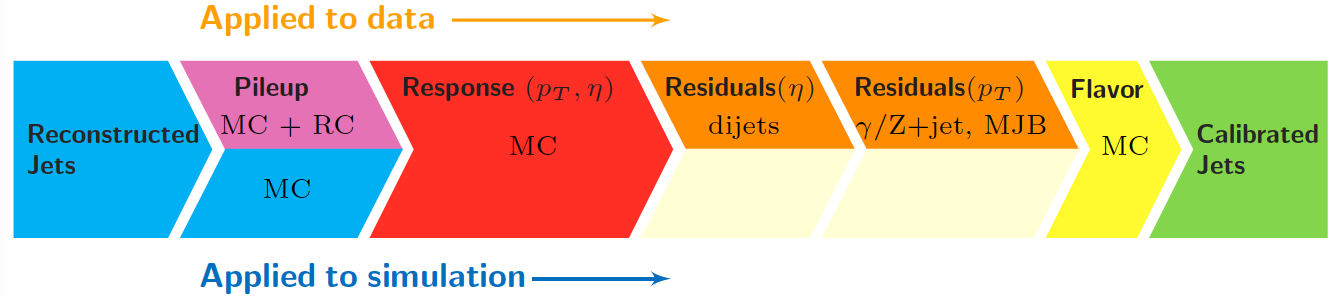
\includegraphics[width=0.9\textwidth]{figuras/Chapter3/JEC_levels.png}
    \caption{Levels of corrections for PF jet four-momentum. Figure taken from \cite{JESandJER}}
    \label{fig:JEC_levels}
  \end{center}
\end{figure}
% Jets are reconstructed with the Particle Flow technique (PF) using the anti$-$k$_{T}$ algorithm \cite{Alwall:2011uj}.
\begin{itemize}
 \item \textbf{Pileup correction}: Also referred as ``L1 corrections''. It corrects the additional tracks and the excess of energy deposits
in the calorimeters due pileup events. The amount of the pile-up contribution
to the jet energy can be estimated from the global per-event $p_{T,offset}$ density 
$\rho$ and the jet area \cite{JECpileup}. This amount is obtained from 
simulated dijet events with and without PU.
 \item \textbf{True response}: The second level of JEC is related to the detector response to hadrons (L2L3 MC-truth corrections), correcting
the non-uniformity in $\eta$ and the non-linearity in $p_{\textrm{T}}$. The simulated jet response is determined
with QCD-multijet events generated with Pythia and with a simulation of the CMS detector based
on Geant4.
 \item \textbf{Residual corrections}: L2L3 Residual corrections are applied in order to address the remaining difference
between the jet response on data and MC (of the order of $1 \%$). This corrections are achieved with data-driven methods, using
dijet samples for $\eta$-dependent corrections and $\gamma /$Z+jets samples for the corrections to $p_{\textrm{T}}$. 
 \item \textbf{Flavor corrections}: The true corrections were performed considering QCD samples with mixture at parton level. 
 Therefore, the flavor correction intends to correct the jet at parton level considering that the jet was produced 
 by an specific parton flavor \cite{CMS-PAS-JME-07-002}. 

\end{itemize}



\section{b-jets Identification}
\label{sec:bJet}
The identification of jets originated from the decay of bottom quarks, i.e. b-tagging, exploits 
the properties of the $B$-hadrons such as their large decay life-times ($c\tau~$450 $\mu$m, which leads
to displaced tracks in the tracker) as well as the presence of leptons in the final 
state due their semileptonic decays. CMS has developed several algorithms for b-jet 
identification \cite{Chatrchyan:2012jua} based on the properties of the $B$-hadron 
decays such as large impact parameter with respect to the primary 
vertex of charged particle tracks, a possible secondary vertex 
reconstructed inside the jet, the mass and the number of tracks associated to the secondary
vertex, the number of tracks in the jet as well as the possible presence of soft leptons. The 
algorithm used in the analyses is the Combined Secondary Vertex (CSV) and shows the best 
performance for b-jet identification \cite{CMS:2013vea}. CSV algorithm makes 
use of Multivariate Variable Analysis (MVA) in order to  
discriminate b-jets, combining the variables based 
on displaced tracks, secondary vertex information and jet kinematics; the method
provides from a likelihood ratio a single discriminator that defines the compatibility of a jet to be originated
from a b-quark. The CSV discriminator defines three possible working points that 
allows to select a high b-tagging efficiency (CSVL, loose working point) or 
a high purity of b-jet samples (CSVT, tight working point); the remaining
working point shows a high efficiency preserving high purity 
(CSVM, middle working point). The three working points are defined 
according to their b-tagging misidentification rate (probability of an non-b jet to be tagged as a b-jet)
and their b-tagging efficiency (probability of a real b-jet to be tagged by the algorithm). Table 
\ref{table:b-tagWP} shows the b-tagging efficiency for the three working points.\\

%\ref{table:b-tagWP} shows the b-tagging misidentification rate and the b-tagging efficiency
%for the three working points.\\

\begin{table}[ht]%[!Hhtbp]
\centering{
% TABLA CON MISTAG PROBABILITY FOR RUN I... NECESITA SER ACTUALIZADA
%  \begin{tabular}{ | c | c | c | c |} \hline 
%             \textbf{Working Point} & \textbf{CSVv2 discriminator} & \textbf{Mistag probability}  & \textbf{b-tagging efficiency} \\ \hline \hline
%	      Loose                 & $\geq$ 0.460               & 10 $\%$                      &  $\approx$ 83 $\%$ \\ \hline
%	      Medium                & $\geq$ 0.800               & 1 $\%$                       &  $\approx$ 69 $\%$ \\ \hline
%	      Tight                 & $\geq$ 0.935               & 0.1 $\%$                     &  $\approx$ 49 $\%$ \\ \hline
%  \end{tabular}
  \begin{tabular}{ | c | c | c |} \hline 
             \textbf{Working Point} & \textbf{CSVv2 discriminator}   & \textbf{b-tagging efficiency} \\ \hline \hline
	      Loose                 & $\geq$ 0.5426                   &  $\approx$ 83 $\%$ \\ \hline
	      Medium                & $\geq$ 0.8484                   &  $\approx$ 69 $\%$ \\ \hline
	      Tight                 & $\geq$ 0.9535                   &  $\approx$ 49 $\%$ \\ \hline
  \end{tabular}

\caption{CSVv2 discriminator threshold and corresponding efficiency for the three working points, using 
b-jets with transverse momentum above 30 GeV in simulated $t\bar{t}$ events with pp collisions 
at $\sqrt{s}=13$ TeV. The numbers of this table can be used as reference since they depends on
$p_{T}$ and $\eta$ distributions of the jets \cite{CMS:2016kkf}.\label{table:b-tagWP}}
}
\end{table}

%Loose (CSVL) ≥ 0.244 10 % 80 %
%Medium (CSVM) ≥ 0.679 1 % 65 %
%Tight (CSVT) ≥ 0.898 0.1 % 50 %


The b-tagging algorithm has been improved for Run II (CSVv2) with the main aim of reducing
%The off-line b-jet identification algorithm has been improved for Run II (CSVv2) with the main aim of reducing
the execution time. CVSv2 includes an updated multivariate algorithm
that makes use of a Neural Network method instead a simple likelihood rate to estimate the CSV discriminator, 
besides it uses a new algorithm for secondary vertex reconstruction (Inclusive Vertex Finder, IVF) as well as   
an improved track selection. The improvement of the CSVv2 algorithm lead to an increase about 10 $\%$ in 
the b-jet identification efficiency compared to the CSV used for Run I \cite{1742-6596-664-8-082055}. See Figure \ref{fig:bjetRun1vsRun2}.

\begin{figure}[ht]%[!Hhtbp]
  \begin{center}
    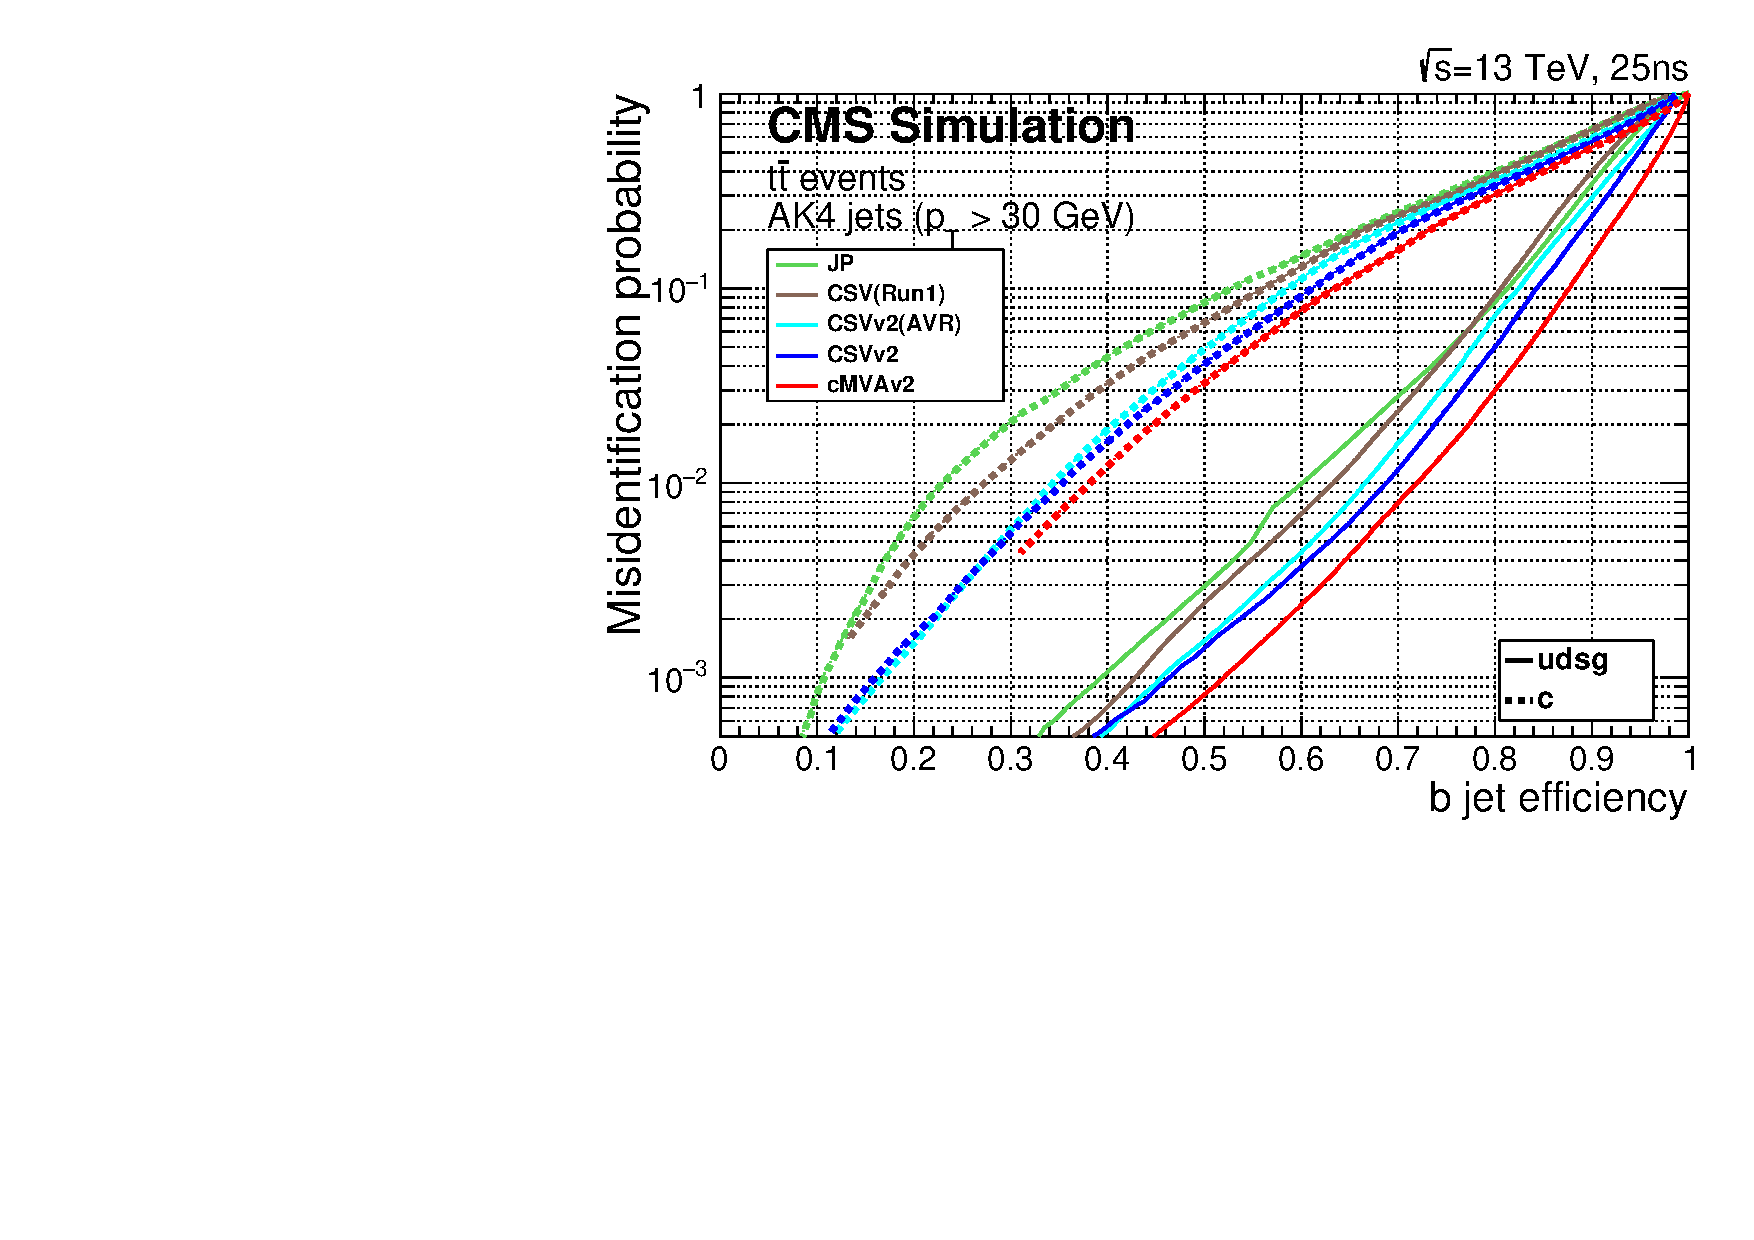
\includegraphics[width=0.6\textwidth]{figuras/Chapter3/bjet_performance_algos.pdf}
    \caption{Efficiency of non-b jets to be misidentified as b-jet as a function of the efficiency to correctly identify
             b-jets for several jet identification algorithms, using enriched $t\bar{t}$ events with 2.6 fb$^{-1}$ of pp 
             collision data collected in 2015 at at $\sqrt{s}=13$ TeV and a BX of 25 ns. Although cMVAv2 algorithm 
             shows the best performance, the CSVv2 algorithm is used for many analysis and shows an improvement compared 
             with the CSV algorithm used in Run I. Figure taken from \cite{CMS:2016kkf}}
    \label{fig:bjetRun1vsRun2}
  \end{center}
\end{figure}

\section{MET}
\label{sec:MET}

%Almost all the final states that come from a pp collision can be detected and
%identified by the CMS sub-systems because of their electromagnetic and/or 
%strong interaction with the detector material. However, neutral particles 
%that only interact weakly with matter, such as the neutrino or the hypothetical neutralino, 
%can scape from the CMS subsystems without detection carr

Almost all the final states coming from a pp collision 
can be measured and identified by the CMS detector with exception 
of neutral particles that only interacts weakly with matter, such as 
the neutrino and the hypothetical neutralino. Although these particles 
scape from CMS without detection, it is possible to infer the 
transverse momenta carried by all of them making use of the 
transverse momentum conservation. The total momentum imbalance in the orthogonal 
plane to the beam line of all detected particles determines the transverse
momentum carried by all weakly interacting particles, also called 
the missing transverse momentum ($\vec{\not{E}_{T}}$). There are several algorithms for 
the $\vec{\not{E}_{T}}$ reconstruction in CMS \cite{Chatrchyan:2011tn}, 
but the most important are: PF $\vec{\not{E}_{T}}$ algorithm which is based on the PF technique 
and the Calo$-\vec{\not{E}_{T}}$ which uses the deposited energy in the calorimeter towers.
The PF $\vec{\not{E}_{T}}$ reconstruction is widely used by the CMS analysis in which PF 
$\vec{\not{E}_{T}}$ is defined as the negative of the vectorial 
sum of transverse momenta of all PF particles, and its module is 
known as missing transverse energy ($\not{E_{T}}$).\\

However, as well as the jet reconstruction, the missing transverse momentum
can be overestimated due to detector responses and experimental effects such 
as pileup, the non-linearity and non-uniformity of the detector response to 
hadrons (see section \ref{sec:Jet}). With the purpose to address the overestimation, 
there are three kinds of corrections can be applied to the $\vec{\not{E}_{T}}$ 
measurement:

\begin{itemize}
 \item \textbf{Type-0 Correction}: Removes the pileup contribution subtracting
 from $\vec{\not{E}_{T}}$ the charged hadrons that might be originated 
 from a pile-up interaction. Besides, it estimates the contribution of neutral 
 hadrons that come from pile-up interactions and removes them from $\vec{\not{E}_{T}}$.

  \item \textbf{Type-I Correction}: This correction makes use of the JEC 
 for the $\vec{\not{E}_{T}}$ reconstruction. It identifies all the particles that can be 
 clustered into jets and replaces their momentum with the sum of the transverse momenta of the 
 jets to which JEC applied:

\begin{equation}
  \label{eq:METcorrection}
  \vec{\not{E_{T}}}^{corr}= \vec{\not{E_{T}}} - \sum_{jets}(\vec{p_{T,jet}^{corr}}-\vec{p_{T,jet}})
\end{equation} 
where ``corr'' refers to the corrected values \cite{CMS-PAS-JME-16-004}. 
 
 \item \textbf{xy-Shift Correction}: the $\not{E}_{T}$ measurement should be independent of $\phi$
 due the cylindrical symmetry of the CMS detector, however a dependency on $\phi$ is observed which 
 might come from anisotropic detector responses, inactive calorimeter cells and detector 
 misalignment. Besides, the $\phi$ dependency on $\not{E}_{T}$ is also correlated with the pileup
 contributions and can be mitigated by shifting the origin of the transverse momentum plane
\end{itemize}

The ``type-I'' correction to $\vec{\not{E}_{T}}$ is widely preferred by CMS analyses. For Run II, 
``type-I'' correction requires jets with $p_{T} >$ 15 GeV (including JEC) which deposited 
energy fraction in the ECAL is less than 0.9 \cite{CMS-PAS-JME-16-004}. \\

The performance and resolution of $\not{E_{T}}$ reconstruction are estimated 
from events which a Z boson is identified (It is also estimated with events 
with an isolated photon). The resolution of $\not{E_{T}}$ is dominated 
by the hadron activity in the event due the high momentum resolution of the leptons, which varies 
from 1-6$\%$ for muons, 1-4$\%$ for eletrons$/$photons and 5-15$\%$ for jets. The Figure FIGURE shows the 
good agreement between data and simulated events for the $\not{E_{T}}$ distribution in the 
 channels $Z\rightarrow \mu^{-}\mu^{+}$ and $Z\rightarrow e^{-}e^{+}$ \cite{CMS-PAS-JME-16-004}.
 %The performance of the $\not{E_{T}}$ reconstruction is measured from a comparison between the momentum of the Z boson with hadron recoil 
 
\begin{figure}[ht]
  \begin{center}
    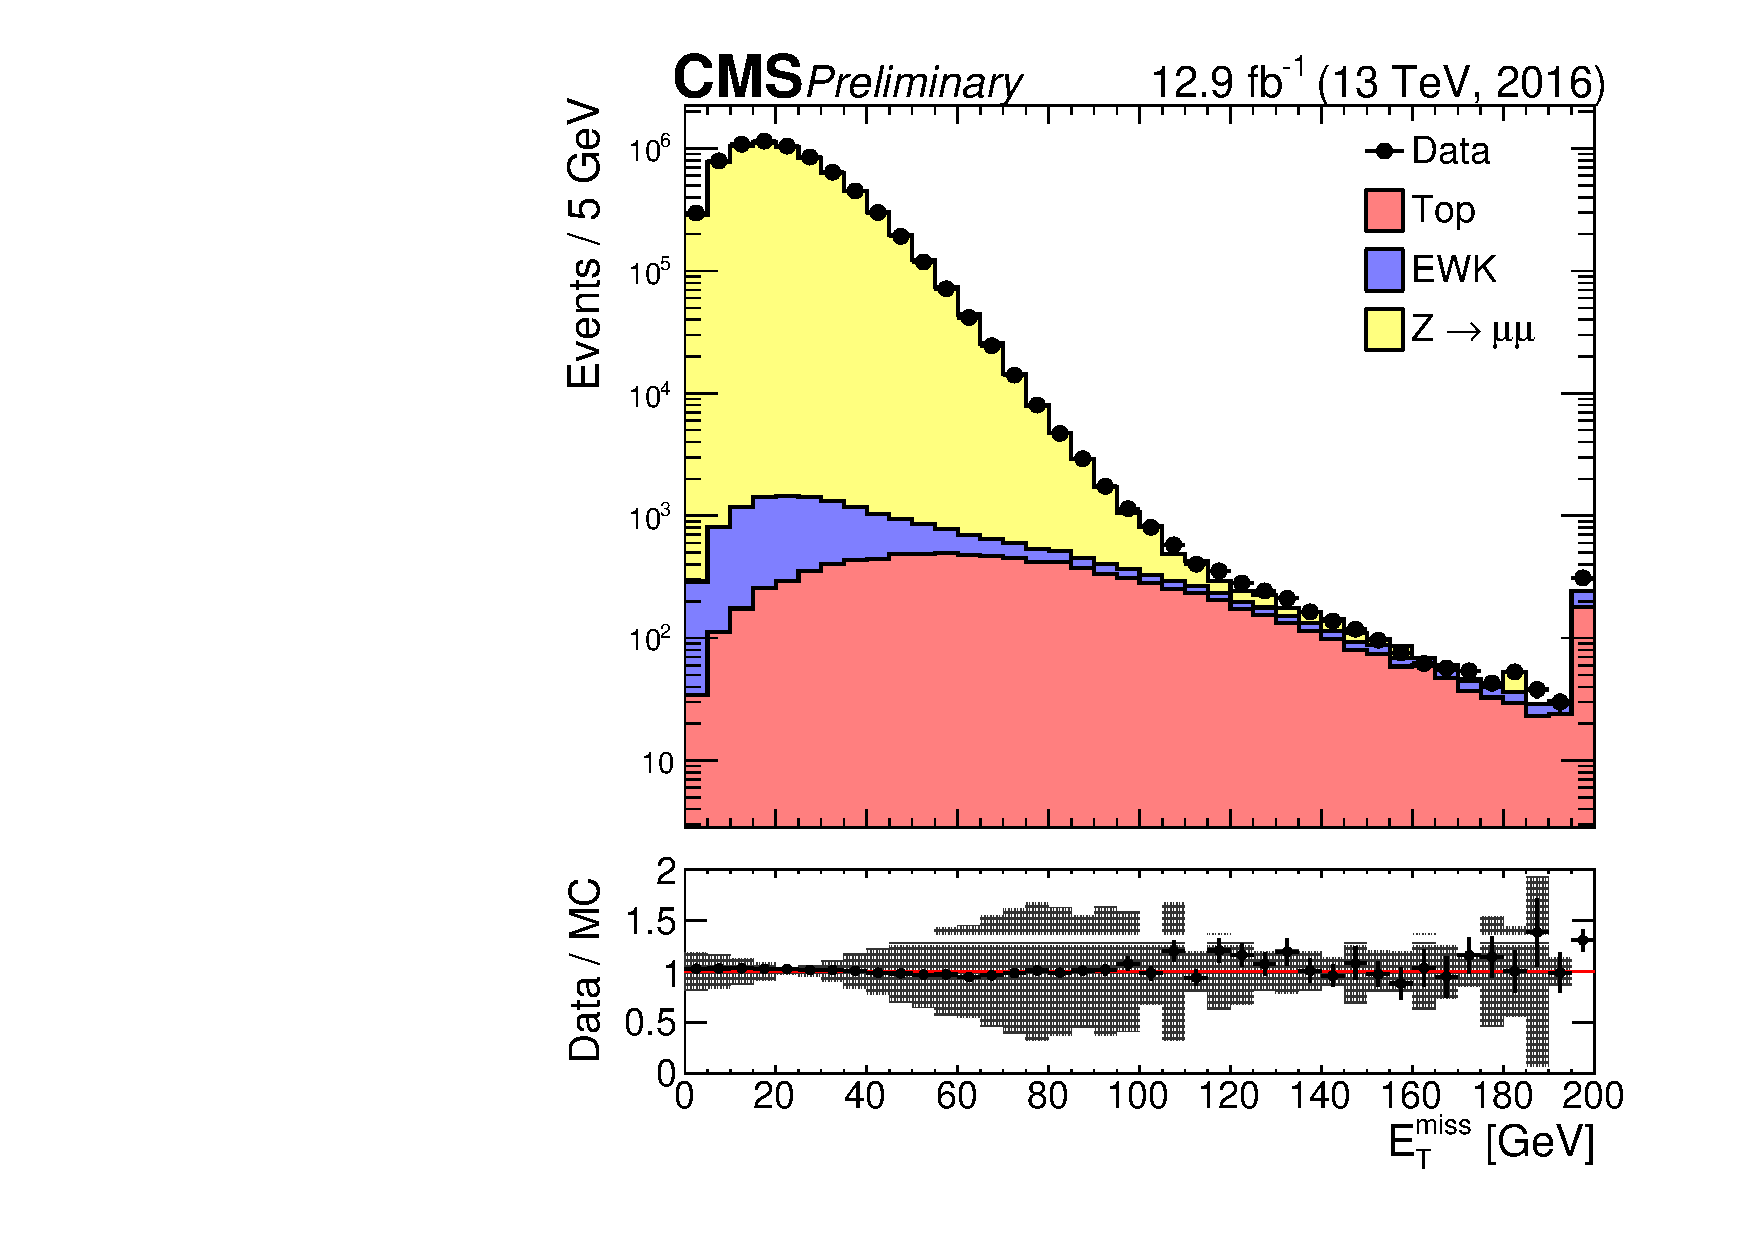
\includegraphics[width=0.43\textwidth]{figuras/Chapter3/METPerformancemumu.pdf}
    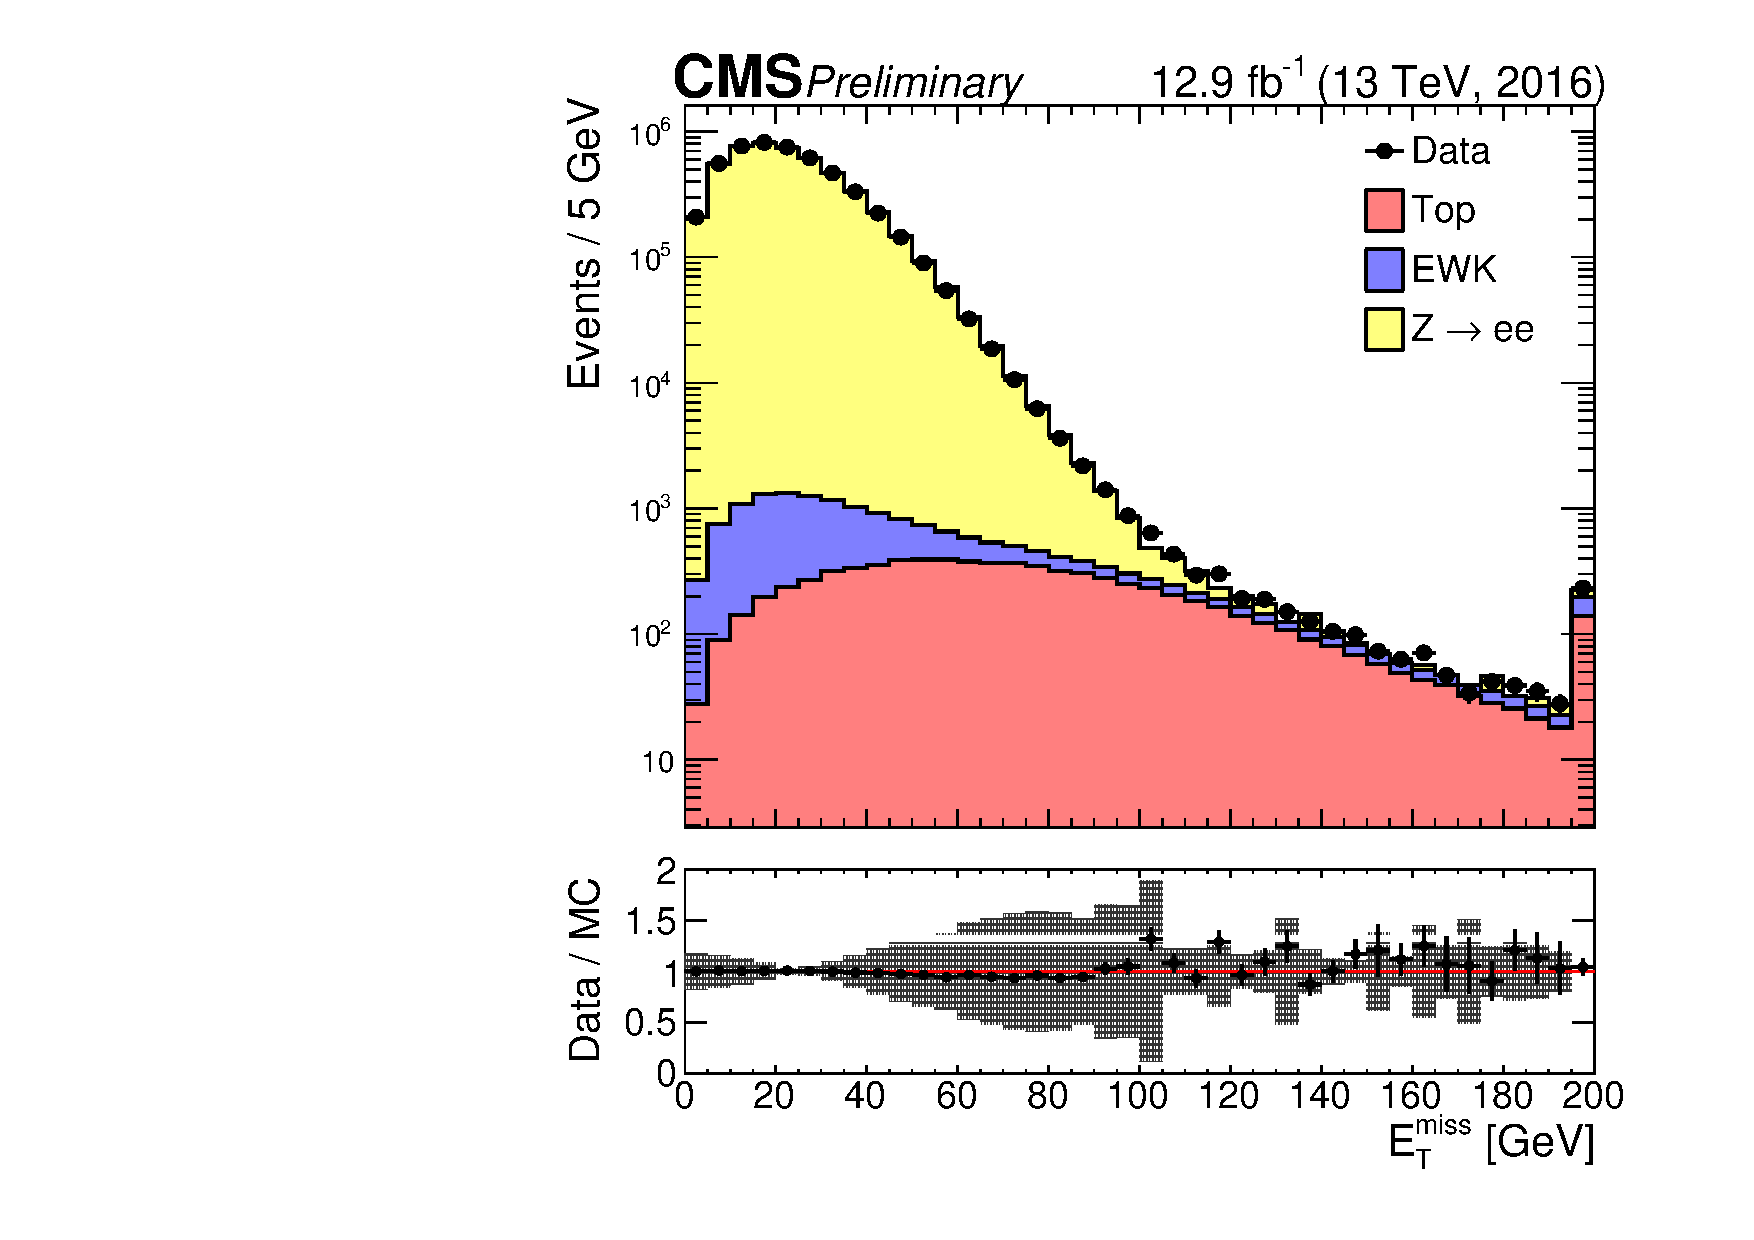
\includegraphics[width=0.43\textwidth]{figuras/Chapter3/METPerformanceee.pdf}
    \caption{$\not{E_{T}}$ distribution for $Z\rightarrow \mu^{-}\mu^{+}$ (left) and $Z\rightarrow e^{-}e^{+}$ (right). Data 
    correspond to pp collisions at 13 TeV collected by CMS detector during 2016 (integrated luminosity up to 12.9 fb$^{-1}$).
    Figure taken from \cite{CMS-PAS-JME-16-004}.}
    \label{fig:MetPerfomance}
  \end{center}
\end{figure} 

%The $\vec{\not{E}_{T}}$ is corrected taking into account those corrections performed to the jet $p_{T}$:

%CMS can be considered as an hermetic detector since almost all the final states 
%coming from a pp collision can be measured and identified, with exception
%of neutral particles that only interacts weakly with matter such as 
%the neutrino and the hypothetical neutralino. Although these particles 
%scape from CMS without detection, it is possible to infer the 
%transverse momenta carried by all of them making use of the 
%transverse momentum conservation. The missing transverse momentum ($E_{T}^{miss}$),
%the momentum (in the orthogonal plane to the beam line) carried by all particles that only interact weakly, is defined
%as the momentum imbalance in the transverse plane to the beam line of all
%particles detected. 



%excluding the region close to the beam
%pipe and the gaps between the various subdetectors and between the di↵erent modules of each



%An efficiency larger than 80% is obtained for jets with a p T > 20 GeV/c. The 100% plateau is reached above
%40 GeV/c, at which point the mismatched jet rate is negligible





%JER Article
%The jet p T resolutions are determined with both dijet and photon+jet events, as discussed in
%section 8. The reference resolutions obtained from simulation are parameterized as a function of
%particle-level jet p T, ptcl (defined in section 2) and average number μ of pileup interactions in bins
%of jet η. Corrections for differences between data and MC simulation are applied as η-binned scale
%factors




%Since in average 85 $\%$ of the constituents of a jet are charged particles and photons, the jet energy resolution

%PF jet momentum and spatial resolutions are greatly improved with respect to calorimeter jets, as
%the use of the tracking detectors and high granularity of the ECAL improves the energy resolution
%through the independent measurements of charged hadrons and photons inside a jet, which together
%2.1constitute ≈85% of the average jet energy. In reconstructing the PF candidate four-momentum,
%photons are assumed massless and charged hadrons are assigned the charged pion mass.

%As mentioned previously, the typical jet energy fractions carried by charged particles, photons
%and neutral hadrons are 65%, 25% and 10% respectively. These fractions ensure that 90% of
%the jet energy can be reconstructed with good precision by the particle-flow algorithm, both in
%value and direction, while only 10% of the energy is affected by the poor hadron calorimeter
%resolution and by calibration corrections of the order of 10 to 20%. As a natural consequence,
%it is expected that jets made of reconstructed particles be much closer to jets made of MonteCarlo–generated
%particles than jets made from the sole calorimeter information, in energy, direction
%and content. It is the purpose of this section to quantify this statement.

%($c\tau > 1$ cm)


%\subsection{Online Identification}
%\label{subsec:JetTrigger}

%\subsection{Offline Identification}
%\label{subsec:JetReconstruction}



%\subsection{Online Identification}
%\label{subsec:ElectronTrigger}

%\subsection{Offline Identification}
%\label{subsec:ElectronReconstruction}

%%%% DEFINED


%\section{Photon Reconstruction}
%\label{sec:Photon}


%\section{Muon Reconstruction}
%\label{sec:Muon}

%\section{Electron Reconstruction}
%\label{sec:Electron}

%\section{B-Jet Reconstruction}
%\label{sec:BJet}



%\section{Tau Lepton}
%\label{sec:Tau}

%\subsection{Tau Reconstruction}
%\label{subsec:TauTrigger}

%\subsection{Tau Reconstruction}
%\label{subsec:TauReconstruction}

%\subsection{Working Points}
%\label{subsec:wp}

%\subsubsection{Efficiency of Working Points}
%\label{subsubsec:Eff_WP}

%\subsection{Fake Rates}
%\label{subsec:FakeRates}

%\subsection{Perspectives Run III}
%\label{subsec:Perspectives} 